\chapter{Specifica dei casi d'uso}

\section{Introduzione}
In questo documento sono analizzati ed elencati gli attori ed i casi d'uso del sistema.
Scopo del documento è la dettagliata descrizione delle modalità di interazione tra le diverse entità presenti ed il sistema.
Ciò permetterà di mettere in evidenza eventuali conflitti tra i requisiti del sistema stesso.
Tale analisi e descrizione dei casi d'uso verrà presentata tramite grafici che seguono lo standard UML.

\noindent
Si utilizzeranno le seguenti convenzioni:
\begin{itemize}
	\item Nei casi in cui più attori possono accedere ad un determinato caso d’uso, ma quest'ultimo è rivolto principalmente ad un solo attore, non verranno elencati tutti gli altri.

	\item Non verranno riportati tutti gli attori che hanno accesso ad un determinato caso d'uso, ma solo l'attore più generico.
	
	\item Nei diagrammi dei casi d'uso non viene riportato l'identificatore del singolo caso d'uso ma solo il titolo, per facilitarne la lettura.
\end{itemize}

\section{Elenco degli attori}
Gli attori che interagiscono con il portale sono elencati di seguito:
\begin{itemize}
	\item \newListItem{att:visitatore}{\formattaAtt}{Visitatore}
	\item \newListItem{att:figuraPubblicaAutenticata}{\formattaAtt}{Figura Pubblica Autenticata}
	\item \newListItem{att:figuraAmministrativa}{\formattaAtt}{Figura Amministrativa}
	\item \newListItem{att:utente}{\formattaAtt}{Utente}
	\item \newListItem{att:produttore}{\formattaAtt}{Produttore}
	\item \newListItem{att:redattore}{\formattaAtt}{Redattore}
	\item \newListItem{att:assistente}{\formattaAtt}{Assistente}
	\item \newListItem{att:moderatore}{\formattaAtt}{Moderatore}
	\item \newListItem{att:amministratore}{\formattaAtt}{Amministratore}
	\item \newListItem{att:cms}{\formattaAtt}{CMS}
\end{itemize}
La gerarchia degli attori è mostrata nel seguente diagramma UML:
\begin{center}
   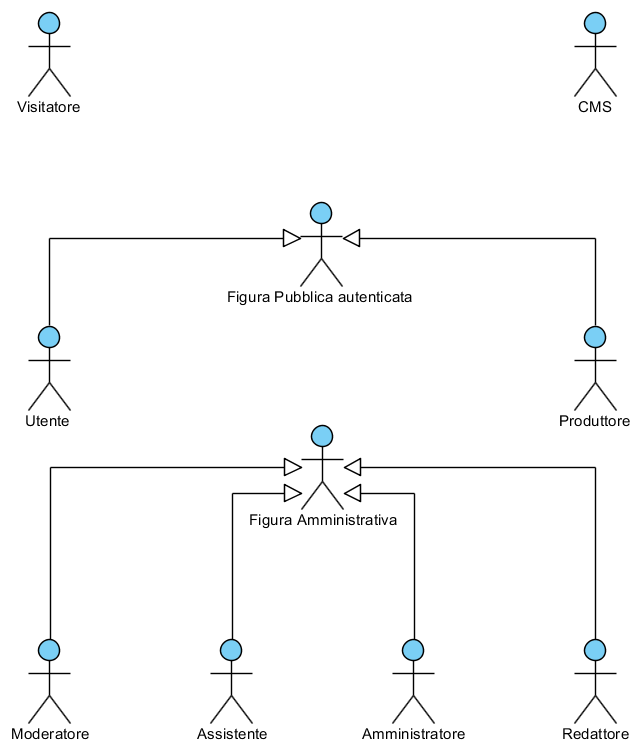
\includegraphics[width=\textwidth]{assets/visualParadigm/SchemaAttori}
\end{center}

\section{Specifica degli attori}
Gli attori che interagiscono con il portale sono descritti di seguito:
\attTab{att:visitatore}{-}{\glsdesc*{visitatore}}

\tabattvspace

\attTab{att:figuraPubblicaAutenticata}{-}{\glsdesc*{figuraPubblicaAutenticata}}

\tabattvspace

\attTab{att:figuraAmministrativa}{-}{\glsdesc*{figuraAmministrativa}}

\tabattvspace

\attTab{att:utente}{\getTitletodesc{att:figuraPubblicaAutenticata}}{\glsdesc*{utente}}

\tabattvspace

\attTab{att:produttore}{\getTitletodesc{att:figuraPubblicaAutenticata}}{\glsdesc*{produttore}}

\tabattvspace

\attTab{att:redattore}{\getTitletodesc{att:figuraAmministrativa}}{\glsdesc*{redattore}}

\tabattvspace

\attTab{att:assistente}{\getTitletodesc{att:figuraAmministrativa}}{\glsdesc*{assistente}}

\tabattvspace

\attTab{att:moderatore}{\getTitletodesc{att:figuraAmministrativa}}{\glsdesc*{moderatore}}

\tabattvspace

\attTab{att:amministratore}{\getTitletodesc{att:figuraAmministrativa}}{\glsdesc*{amministratore}}

\tabattvspace

\attTab{att:cms}{-}{\glsdesc*{cmsdef}}

\section{Identificativo dei casi d'uso} %(vengono usati per definire l'ID, non ha senso metterli dopo la struttura ID)
Di seguito è spiegato come interpretare l'identificativo dei casi d'uso:
\begin{center}
	\use{categoria}{caso}%{[sottoreq]}{[\dots]}
\end{center}

\noindent
Segue una descrizione di ogni campo utilizzato nell'identificatore:
\begin{itemize}
	\item La \campiIdReq{categoria} è una lettera utilizzata per raggruppare i casi d'uso con scopi simili.
	Le categorie sono le seguenti:
	\begin{enumerateIndLabel}{\textsf{\Alph*}}{\Alph*}
		\item Autenticazione. \label{pkg:autenticazione}
		\item Gestione iscrizioni. \label{pkg:iscrizione}
		\item Gestione vetrina. \label{pkg:vetrina} 
		\item Gestione notizie. \label{pkg:notizie}
		\item Gestione suggerimenti. \label{pkg:suggerimenti}
		\item Gestione account. \label{pkg:account}
		\item Gestione valutazioni. \label{pkg:gestionevalutazione}
		\item Gestione recensioni. \label{pkg:gestionerecensione}
		\item Interazione tra figure. \label{pkg:interazione}
		\item Gestione ticket. \label{pkg:gestioneticket}
		\item Ricerca contenuti. \label{pkg:ricerca}
		\item Gestione prodotti mancanti. \label{pkg:prodottimancanti}
		\item Visualizzazione contenuti pubblici. \label{pkg:visualizzazione}
	\end{enumerateIndLabel}

	\item Il campo \campiIdReq{caso} è un numero progressivo utilizzato per identificare in modo univoco un caso d'uso all'interno della sua categoria.
\end{itemize}

\section{Elenco dei casi d'uso}
Vengono di seguito elencati i casi d'uso:
\begin{itemize} 
	\setCatCU{\ref*{pkg:autenticazione}}%A
	\item \newListItem{cu:login}{\formattaCU}{Login}
	\item \newListItem{cu:loginAmm}{\formattaCU}{Login Figure Amministrative}
	\item \newListItem{cu:logout}{\formattaCU}{Logout}

	\setCatCU{\ref*{pkg:iscrizione}}%B
	\item \newListItem{cu:iscrizionePortale}{\formattaCU}{Iscrizione tramite modulo}
	\item \newListItem{cu:iscrizioneSocial}{\formattaCU}{Iscrizione tramite Social Network}
	\item \newListItem{cu:iscrizioneApprovazione}{\formattaCU}{Iscrizione tramite approvazione}
	\item \newListItem{cu:approvazioneIscrizione}{\formattaCU}{Approvazione iscrizione}

	\setCatCU{\ref*{pkg:vetrina}}%C
	\item \newListItem{cu:personalizzaVetrinaInsDesc}{\formattaCU}{Inserimento descrizione}
	\item \newListItem{cu:personalizzaVetrinaModDesc}{\formattaCU}{Modifica descrizione}
	\item \newListItem{cu:personalizzaVetrinaInsImg}{\formattaCU}{Inserimento immagine}
	\item \newListItem{cu:personalizzaVetrinaDelImg}{\formattaCU}{Rimozione immagine}
	\item \newListItem{cu:personalizzaVetrinaInsProd}{\formattaCU}{Inserimento prodotto}
	\item \newListItem{cu:personalizzaVetrinaModProd}{\formattaCU}{Modifica prodotto}
	\item \newListItem{cu:statistichePrivateVetrina}{\formattaCU}{Visualizzazione statistiche private della vetrina}


	\setCatCU{\ref*{pkg:notizie}}%D
	\item \newListItem{cu:inserimentoNotizia}{\formattaCU}{Inserimento notizia}
	\item \newListItem{cu:modificaNotizia}{\formattaCU}{Modifica notizia}
	\item \newListItem{cu:rimozioneNotizia}{\formattaCU}{Rimozione notizia}

	\setCatCU{\ref*{pkg:suggerimenti}}%E
	\item \newListItem{cu:suggerimentoProdotti}{\formattaCU}{Suggerimento prodotti}
	\item \newListItem{cu:notizieSimili}{\formattaCU}{Suggerimento notizie simili}
	
	\setCatCU{\ref*{pkg:account}}%F
	\item \newListItem{cu:accessoProfilo}{\formattaCU}{Accesso al proprio profilo}
	\item \newListItem{cu:modificaImpostazioni}{\formattaCU}{Modifica delle proprie impostazioni}
	\item \newListItem{cu:rimozioneAccountProprio}{\formattaCU}{Rimozione account proprio}

	\item \newListItem{cu:rimozioneAccountAltrui}{\formattaCU}{Rimozione account altrui}
	\item \newListItem{cu:modificaPrivilegiAccount}{\formattaCU}{Modifica privilegi di un account}
	%\item \newListItem{cu:aggiungiPrivilegiAccount}{\formattaCU}{Aggiungi privilegi ad account}
	%\item \newListItem{cu:rimuoviPrivilegiAccount}{\formattaCU}{Rimuovi privilegi da account}

	\setCatCU{\ref*{pkg:gestionevalutazione}}%G
	\item \newListItem{cu:inserisciValutazioneProdotto}{\formattaCU}{Inserimento valutazione}
	\item \newListItem{cu:modificaValutazioneProdotto}{\formattaCU}{Modifica valutazione}

	\setCatCU{\ref*{pkg:gestionerecensione}}%H
	\item \newListItem{cu:inserisciRecensioneProdotto}{\formattaCU}{Inserimento recensione}
	\item \newListItem{cu:modificaRecensioneProdotto}{\formattaCU}{Modifica recensione propria}
	\item \newListItem{cu:eliminaRecensioneProdotto}{\formattaCU}{Rimozione recensione propria}
	\item \newListItem{cu:commentoRecensione}{\formattaCU}{Commento a recensione}
	\item \newListItem{cu:giudizioRecensione}{\formattaCU}{Giudizio recensione}
	\item \newListItem{cu:modificaGiudizioRecensione}{\formattaCU}{Modifica giudizio recensione}
	\item \newListItem{cu:segnalazioneContenutiInap}{\formattaCU}{Segnalazione contenuti inappropriati}
	\item \newListItem{cu:mostraSegnContenutiInap}{\formattaCU}{Visualizzazione segnalazioni contenuti}
	\item \newListItem{cu:rimozioneContenutiInap}{\formattaCU}{Rimozione contenuti inappropriati}

	\setCatCU{\ref*{pkg:interazione}}%I
	\item \newListItem{cu:followAccount}{\formattaCU}{Follow account}
	\item \newListItem{cu:unFollowAccount}{\formattaCU}{Unfollow account}

	\setCatCU{\ref*{pkg:gestioneticket}}%J
	\item \newListItem{cu:ticketInvio}{\formattaCU}{Invio di un ticket}
	\item \newListItem{cu:ticketRisposta}{\formattaCU}{Risposta ad un ticket}
	\item \newListItem{cu:ticketChiudi}{\formattaCU}{Chiusura di un ticket}
	\item \newListItem{cu:ticketLettura}{\formattaCU}{Lettura di un ticket}

	\setCatCU{\ref*{pkg:ricerca}}%K
	\item \newListItem{cu:ricercaProdotto}{\formattaCU}{Ricerca prodotto}
	%\item \newListItem{cu:selezionaProdotto}{\formattaCU}{Seleziona prodotto}
	\item \newListItem{cu:ricercaProfilo}{\formattaCU}{Ricerca profilo}
	%\item \newListItem{cu:selezionaProfilo}{\formattaCU}{Seleziona profilo}
	\item \newListItem{cu:ricercaNotizia}{\formattaCU}{Ricerca notizia}
	%\item \newListItem{cu:selezionaNotizia}{\formattaCU}{Seleziona notizia}

	\setCatCU{\ref*{pkg:prodottimancanti}}%L
	\item \newListItem{cu:richiestaInsProdotto}{\formattaCU}{Richiesta inserimento prodotto}
	\item \newListItem{cu:mostraRichiestaInsProdotto}{\formattaCU}{Visualizzazione richiesta prodotto}
	\item \newListItem{cu:richiestaInsProduttore}{\formattaCU}{Richiesta inserimento produttore e prodotto}

	\setCatCU{\ref*{pkg:visualizzazione}}%M
	\item \newListItem{cu:mostraVetrina}{\formattaCU}{Mostra vetrina}
	%\item \newListItem{cu:mostraInfoVetrina}{\formattaCU}{Mostra informazioni vetrina}
%%	\item \newListItem{cu:mostraProdottiVetrina}{\formattaCU}{Mostra prodotti esposti in vetrina}
	\item \newListItem{cu:mostraProdotto}{\formattaCU}{Mostra prodotto}
%	\item \newListItem{cu:mostraAnteprimaProdotto}{\formattaCU}{Mostra anteprima prodotto}
%	\item \newListItem{cu:mostraInfoProdotto}{\formattaCU}{Mostra informazioni del prodotto}
	\item \newListItem{cu:mostraRecProdotto}{\formattaCU}{Mostra recensioni associate al prodotto}
%	\item \newListItem{cu:mostraStatProdotto}{\formattaCU}{Mostra statistiche del prodotto}
	\item \newListItem{cu:mostraProfilo}{\formattaCU}{Mostra profilo pubblico}
%	\item \newListItem{cu:mostraAnteprimaProfilo}{\formattaCU}{Mostra anteprima profilo}
%	\item \newListItem{cu:mostraInfoProfilo}{\formattaCU}{Mostra informazioni di un profilo pubblico}
%	\item \newListItem{cu:mostraStatProfilo}{\formattaCU}{Mostra statistiche di un profilo pubblico}
	\item \newListItem{cu:mostraNotizia}{\formattaCU}{Mostra notizia}
%	\item \newListItem{cu:mostraAnteprimaNotizia}{\formattaCU}{Mostra anteprima notizia}
	\item \newListItem{cu:mostraAggF}{\formattaCU}{Mostra aggiornamenti dai followed}
\end{itemize}	

%{id}{attori}{pre}{post}{flusso}
\section{Specifica dei casi d'uso}
Vengono di seguito elencate le tabelle che descrivono i casi d'uso, suddivisi per categoria:

\subsection{Autenticazione}
\begin{center}
   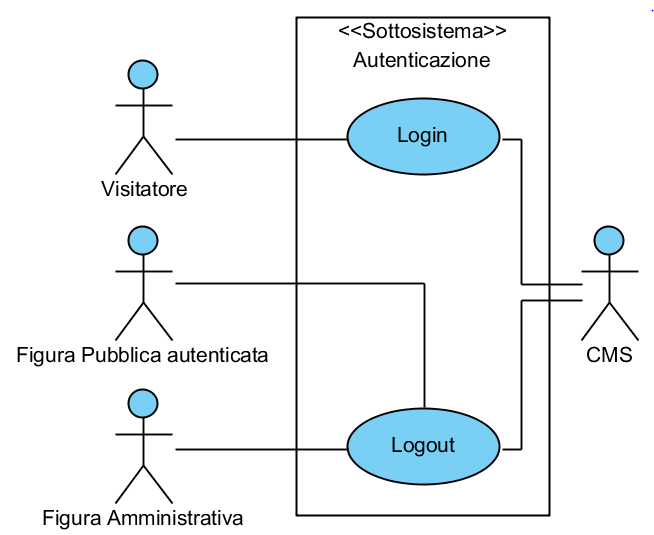
\includegraphics[width=\textwidth]{assets/visualParadigm/Autenticazione}
\end{center}
%*************** LOGIN *****************
\cuTab{cu:login}%
{\getTitletodesc{att:visitatore}}%
{La persona connessa al sito è inizialmente riconosciuta come Visitatore}%
{La persona connessa al sito è ora riconosciuta come Figura Pubblica Autenticata}%
{\begin{enumCU}
	\item Il caso d'uso ha inizio quando un Visitatore richiede di effettuare il login 
	\item Il sistema richiede le credenziali di autenticazione
	\item Il Visitatore inserisce le credenziali di accesso negli appositi campi \label{culogin:3}
	\item Il Visitatore conferma i dati inseriti
	\item Il sistema verifica che i dati inseriti corrispondano ad un account pubblico esistente\label{culogin:5}
	\item Il sistema accetta le credenziali ricevute
\end{enumCU}}%
%
\cuAlternativo{cu:login}
{Flusso alternativo 1}%
{Errore Login}%
{La persona connessa al sito è inizialmente riconosciuta come Visitatore}%
{\postNulle}%
{\begin{enumCU}
	\item Dopo il punto \ref{culogin:5} il sistema rifiuta le credenziali
\end{enumCU}}%
%
\cuAlternativo{cu:login}
{Flusso alternativo 2}%
{Annulla Login}%
{La persona connessa al sito è inizialmente riconosciuta come Visitatore}%
{\postNulle}%
{\begin{enumCU}
		\item Dopo il punto \ref{culogin:3} il Visitatore annulla l'operazione di login
\end{enumCU}}%

\tabcuvspace

\cuTab{cu:loginAmm}%
{\getTitletodesc{att:visitatore}}%
{La persona connessa al sito è inizialmente riconosciuta come Visitatore}%
{La persona connessa al sito è ora riconosciuta come Figura Amministrativa}%
{\begin{enumCU}
	\item Il caso d'uso ha inizio quando un Visitatore richiede di effettuare il login 
	\item Il sistema richiede le credenziali di autenticazione
	\item Il Visitatore inserisce le credenziali di accesso negli appositi campi \label{culoginamm:3}
	\item Il Visitatore conferma i dati inseriti
	\item Il sistema verifica che i dati inseriti corrispondano ad un account amministrativo esistente\label{culoginamm:5}
	\item Il sistema accetta le credenziali ricevute
	\item Il sistema invia un codice casuale sul cellulare del Visitatore
	\item Il Visitatore inserisce il codice ricevuto sul cellulare in un apposito campo \label{culoginamm:8}
	\item Il Visitatore conferma il codice inserito
	\item Il sistema verifica che il codice inserito corrisponda a quello inviato \label{culoginamm:10}
	\item Il sistema accetta il codice ricevuto
\end{enumCU}}%
%
\cuAlternativo{cu:loginAmm}
{Flusso alternativo 1}%
{Errore Credenziali}%
{La persona connessa al sito è inizialmente riconosciuta come Visitatore}%
{\postNulle}%
{\begin{enumCU}
	\item Dopo il punto \ref{culoginamm:5} il sistema rifiuta le credenziali
\end{enumCU}}%
%
\cuAlternativo{cu:loginAmm}
{Flusso alternativo 2}%
{Annulla Credenziali}%
{La persona connessa al sito è inizialmente riconosciuta come Visitatore}%
{\postNulle}%
{\begin{enumCU}
		\item Dopo il punto \ref{culoginamm:3} il Visitatore annulla l'operazione di login
\end{enumCU}}%
%
\cuAlternativo{cu:loginAmm}
{Flusso alternativo 3}%
{Errore Codice}%
{La persona connessa al sito è inizialmente riconosciuta come Visitatore}%
{\postNulle}%
{\begin{enumCU}
		\item Dopo il punto \ref{culoginamm:10}, il sistema rifiuta il codice
\end{enumCU}}%
%
\cuAlternativo{cu:loginAmm}
{Flusso alternativo 4}%
{Annulla Codice}%
{La persona connessa al sito è inizialmente riconosciuta come Visitatore}%
{\postNulle}%
{\begin{enumCU}
		\item Dopo il punto \ref{culoginamm:8}, il Visitatore annulla l'operazione di login
\end{enumCU}}%

\tabcuvspace

%*************** LOGOUT *****************
\cuTab{cu:logout}
{\getTitletodesc{att:figuraAmministrativa}, \getTitletodesc{att:figuraPubblicaAutenticata}}
{La persona connessa al sito è autenticata}
{La persona connessa al sito non è più autenticata ed è ora un Visitatore}
{\begin{enumCU}
	\item Il caso d'uso ha inizio quando una persona autenticata richiede di effettuare il logout
	\item Il sistema effettua il logout richiesto
\end{enumCU}}

\subsection{Gestione iscrizioni}
\begin{center}
   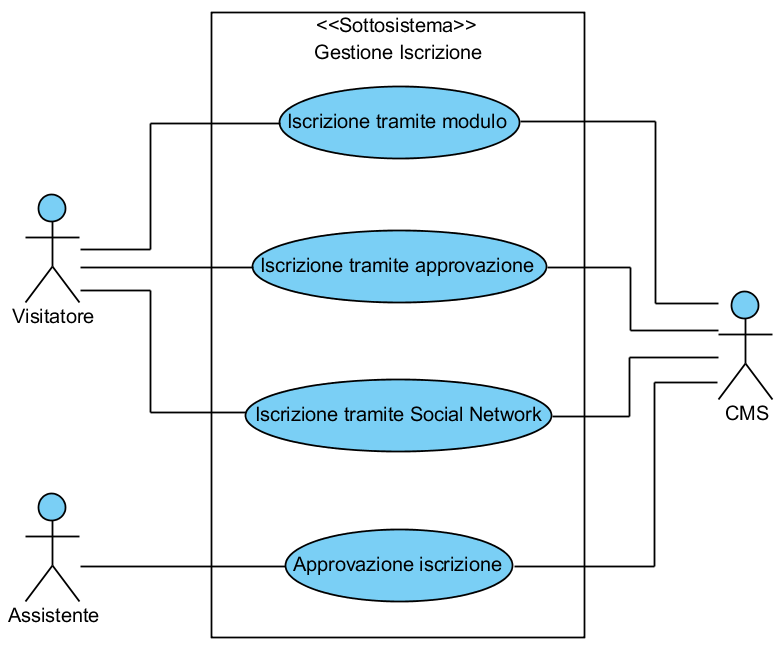
\includegraphics[width=\textwidth]{assets/visualParadigm/GestioneIscrizione}
\end{center}
%*************** ISCRIZIONE PORTALE *****************
\cuTab{cu:iscrizionePortale}
{\getTitletodesc{att:visitatore}}
{La persona connessa al sito è inizialmente riconosciuta come Visitatore}
{La persona ha ora un account proprio, creato con i dati da essa inseriti}
{\begin{enumCU}
	\item Il caso d'uso ha inizio quando un Visitatore richiede di effettuare l'iscrizione
	\item Il sistema richiede i dati richiesti per effettuare l'iscrizione tra cui un identificatore all'interno del sistema
	\item Il Visitatore inserisce i dati richiesti negli appositi campi \label{cuiscr:3}
	\item Il Visitatore conferma i dati inseriti
	\item Il sistema verifica che i dati inseriti siano corretti e che l'identificatore dell'account che si sta creando non sia già presente \label{cuiscr:5}
	\item Il sistema crea un nuovo account con le credenziali ricevute
\end{enumCU}}
%
\cuAlternativo{cu:iscrizionePortale}
{Flusso alternativo 1}%
{Annulla iscrizione}%
{La persona connessa al sito è inizialmente riconosciuta come Visitatore}%
{\postNulle}%
{\begin{enumCU}
		\item Dopo il punto \ref{cuiscr:3} l'utente annulla l'operazione di iscrizione
	\end{enumCU}}%
%
\cuAlternativo{cu:iscrizionePortale}
{Flusso alternativo 2}%
{Errore iscrizione}%
{La persona connessa al sito è inizialmente riconosciuta come Visitatore}%
{\postNulle}%
{\begin{enumCU}
		\item Dopo il punto \ref{cuiscr:5} il sistema rileva un errore nei dati inseriti
	\end{enumCU}}%


\tabcuvspace

%%%FORSE DA TOGLIERE -------------------------------------------------------------------------
%Accorpa verificati e non verificati
\cuTab{cu:iscrizioneSocial}
{\getTitletodesc{att:visitatore}}
{La persona è connessa al sito come Visitatore}
{La persona ha ora un account proprio, creato tramite le API messe a disposizione dal Social Network utilizzato durante l'iscrizione}
{\begin{enumCU}
		\item Il caso d'uso ha inizio quando un Visitatore richiede di effettuare l'iscrizione tramite un Social Network
		\item Il sistema richiede le credenziali di accesso del Social Network scelto
		\item Il Visitatore inserisce i dati richiesti \label{cuiscrappsocial:3}
		\item Il Visitatore conferma i dati inseriti \label{cuiscrappsocial:5}
		\item Il Il sistema crea un nuovo account con le credenziali ricevute
	\end{enumCU}}

\tabcuvspace
%
\cuAlternativo{cu:iscrizioneSocial}
{Flusso alternativo 1}%
{Annulla iscrizione}%
{La persona connessa al sito è inizialmente riconosciuta come Visitatore}%
{\postNulle}%
{\begin{enumCU}
		\item Dopo il punto \ref{cuiscrappsocial:3} il Visitatore annulla l'operazione di iscrizione
	\end{enumCU}}%
%
\cuAlternativo{cu:iscrizioneSocial}
{Flusso alternativo 2}%
{Errore iscrizione}%
{La persona connessa al sito è inizialmente riconosciuta come Visitatore}%
{\postNulle}%
{\begin{enumCU}
		\item Dopo il punto \ref{cuiscrappsocial:5} il sistema rileva un errore nei dati inseriti
	\end{enumCU}}%

\tabcuvspace

%*************** ISCRIZIONE CON APPROVAZIONE *****************
\cuTab{cu:iscrizioneApprovazione}
{\getTitletodesc{att:visitatore}}
{La persona connessa al sito è inizialmente riconosciuta come Visitatore}
{Viene inserita nel sistema una richiesta di creazione di un account di tipo Produttore}
{\begin{enumCU}
	\item Il caso d'uso ha inizio quando un Visitatore richiede di effettuare l'iscrizione tramite approvazione
	\item Il sistema richiede i dati richiesti per effettuare l'iscrizione  tra cui un identificatore all'interno del sistema
	\item Il Visitatore inserisce i dati richiesti negli appositi campi \label{cuiscrapp:3}
	\item Il Visitatore conferma i dati inseriti
	\item Il sistema verifica che i dati inseriti siano corretti e che l'identificatore dell'account che si sta creando non sia già presente \label{cuiscrapp:5}
	\item Il sistema crea una richiesta di iscrizione con le credenziali ricevute
\end{enumCU}}
%
\cuAlternativo{cu:iscrizioneApprovazione}
{Flusso alternativo 1}%
{Annulla iscrizione}%
{La persona connessa al sito è inizialmente riconosciuta come Visitatore}%
{\postNulle}%
{\begin{enumCU}
		\item Dopo il punto \ref{cuiscrapp:3} il Visitatore annulla l'operazione di iscrizione
	\end{enumCU}}%
%
\cuAlternativo{cu:iscrizioneApprovazione}
{Flusso alternativo 2}%
{Errore iscrizione}%
{La persona connessa al sito è inizialmente riconosciuta come Visitatore}%
{\postNulle}%
{\begin{enumCU}
		\item Dopo il punto \ref{cuiscrapp:5} il sistema rileva un errore nei dati inseriti
	\end{enumCU}}%

\tabcuvspace

%***************  APPROVAZIONE DI UNA RICHIESTA DI ISCRIZIONE *****************
\cuTab{cu:approvazioneIscrizione}
{\getTitletodesc{att:assistente}}
{La persona connessa al sito è autenticata e ha i privilegi di  Assistente. Nel sistema è presente almeno una richiesta di creazione di un account}
{Il Visitatore che ha effettuato la richiesta ha ora un account di tipo produttore. Nel sistema non è più presente la richiesta}
{\begin{enumCU}
	\item Il caso d'uso ha inizio quando una persona con privilegi di Assistente richiede di controllare una richiesta di iscrizione
	\item Il sistema mostra all'Assistente le richieste presenti nel sistema e chiede di selezionarne una\label{cuappriscr:0}
	\item L'Assistente seleziona una richiesta di iscrizione
	\item Il sistema mostra all'Assistente la richiesta da lui selezionata\label{cuappriscr:1}
	\item L'Assistente approva la richiesta di iscrizione
\end{enumCU}}
%
\cuAlternativo{cu:approvazioneIscrizione}
{Flusso alternativo 1}%
{Richiesta rifiutata}%
{La persona connessa al sito è autenticata e ha i privilegi di  Assistente. Nel sistema è presente almeno una richiesta di creazione di un account}%
{Nel sistema c'è una richiesta in meno}%
{\begin{enumCU}
		\item Dopo il punto \ref{cuappriscr:1} l'Assistente rifiuta la richiesta di creazione dell'account
		\item Il sistema elimina la richiesta selezionata dall'Assistente
\end{enumCU}}%
%
\cuAlternativo{cu:approvazioneIscrizione}
{Flusso alternativo 2}%
{Annulla operazione di selezione}%
{La persona connessa al sito è autenticata e ha i privilegi di  Assistente. Nel sistema è presente almeno una richiesta di creazione di un account}%
{\postNulle}%
{\begin{enumCU}
		\item Dopo il punto \ref{cuappriscr:0} l'Assistente annulla la selezione
\end{enumCU}}%

\subsection{Gestione vetrina}
\begin{center}
   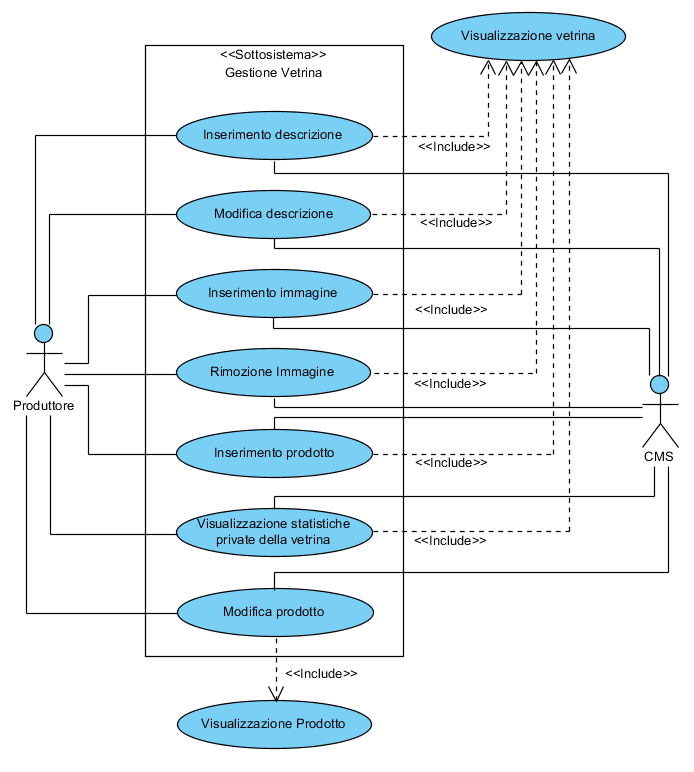
\includegraphics[width=\textwidth]{assets/visualParadigm/GestioneVentrina}
\end{center}
%***************  INSERISCI DESCRIZIONE IN VETRINA *****************
\cuTab{cu:personalizzaVetrinaInsDesc}
{\getTitletodesc{att:produttore}}
{La persona connessa al sito è autenticata e ha i privilegi di Produttore. Nel sistema non è presente la descrizione della vetrina di quel Produttore}
{Nel sistema è presente la descrizione della vetrina del Produttore}
{\begin{enumCU}
		\item Il caso d'uso ha inizio quando un Produttore visualizza la sua vetrina, \inc{cu:mostraVetrina}
		\item Il Produttore richiede di inserire la descrizione della sua vetrina
		\item Il sistema richiede il testo da inserire come descrizione 
		\item Il Produttore inserisce la descrizione nell'apposito campo\label{cuinsdescr:2}
		\item Il Produttore conferma il testo inserito
		\item Il sistema memorizza il testo inserito
	\end{enumCU}}
%
\cuAlternativo{cu:personalizzaVetrinaInsDesc}
{Flusso alternativo 1}%
{Annulla inserimento}%
{La persona connessa al sito è autenticata e ha i privilegi di Produttore. Nel sistema non è presente la descrizione della vetrina di quel Produttore}%
{\postNulle}%
{\begin{enumCU}
		\item Dopo il punto \ref{cuinsdescr:2} il Produttore annulla l'inserimento della descrizione
	\end{enumCU}}%

\tabcuvspace

\cuTab{cu:personalizzaVetrinaModDesc}
{\getTitletodesc{att:produttore}}
{La persona connessa al sito è autenticata e ha i privilegi di Produttore. Nel sistema è presente la descrizione della vetrina di quel Produttore}
{Nel sistema è presente la descrizione della vetrina del Produttore}
{\begin{enumCU}
		\item Il caso d'uso ha inizio quando un Produttore visualizza la sua vetrina, \inc{cu:mostraVetrina}
		\item Il Produttore richiede di modificare la descrizione della sua vetrina
		\item Il sistema richiede il testo da inserire come descrizione, il campo in cui inserire il testo è precompilato con la descrizione già presente nel sistema 
		\item Il Produttore inserisce la descrizione nell'apposito campo\label{cumoddescr:2}
		\item Il Produttore conferma il testo inserito
		\item Il sistema memorizza il testo inserito
	\end{enumCU}}
%
\cuAlternativo{cu:personalizzaVetrinaModDesc}
{Flusso alternativo 1}%
{Annulla modifica}%
{La persona connessa al sito è autenticata e ha i privilegi di Produttore. Nel sistema è presente la descrizione della vetrina di quel Produttore}%
{\postNulle}%
{\begin{enumCU}
		\item Dopo il punto \ref{cumoddescr:2} il Produttore annulla la modifca della descrizione
	\end{enumCU}}%

\tabcuvspace

%***************  INSERISCI IMMAGINE IN VETRINA *****************
\cuTab{cu:personalizzaVetrinaInsImg}
{\getTitletodesc{att:produttore}}
{La persona connessa al sito è autenticata e ha i privilegi di Produttore}
{Nel sistema è presente l'immagine della vetrina del Produttore}
{\begin{enumCU}
		\item Il caso d'uso ha inizio quando un Produttore visualizza la sua vetrina, \inc{cu:mostraVetrina}
		\item Il Produttore richiede di inserire l'immagine della vetrina
		\item Il sistema richiede il percorso nel file system, o nella rete, dell'immagine da inserire 
		\item Il Produttore inserisce il percorso dell'immagine nell'apposito campo\label{cuinsimm:2}
		\item Il Produttore conferma il percorso dell'immagine inserito\label{cuinsimm:3}
		\item Il sistema scarica e memorizza l'immagine impostandola come immagine della vetrina del Produttore
	\end{enumCU}}
%
\cuAlternativo{cu:personalizzaVetrinaInsImg}
{Flusso alternativo 1}%
{Errore inserimento}%
{La persona connessa al sito è autenticata e ha i privilegi di Produttore}%
{\postNulle}%
{\begin{enumCU}
		\item Dopo il punto \ref{cuinsimm:3} il sistema non riesce a trovare, scaricare o inserire correttamente l'immagine
	\end{enumCU}}%
%
\cuAlternativo{cu:personalizzaVetrinaInsImg}
{Flusso alternativo 2}%
{Annulla inserimento}%
{La persona connessa al sito è autenticata e ha i privilegi di Produttore}%
{\postNulle}%
{\begin{enumCU}
		\item Dopo il punto \ref{cuinsimm:2} il produttore annulla l'inserimento dell'immagine
	\end{enumCU}}%

\tabcuvspace

\cuTab{cu:personalizzaVetrinaDelImg}
{\getTitletodesc{att:produttore}}
{La persona connessa al sito è autenticata e ha i privilegi di Produttore. Nel sistema è presente l'immagine della vetrina del Produttore}
{Nel sistema non è presente l'immagine della vetrina del Produttore}
{\begin{enumCU}
		\item Il caso d'uso ha inizio quando un Produttore visualizza la sua vetrina, \inc{cu:mostraVetrina}
		\item Il  Produttore richiede di rimuovere l'immagine della vetrina
		\item Il sistema richiede di confermare l'operazione \label{cudelimm:2}
		\item Il Produttore conferma l'operazione
		\item Il sistema rimuove l'immagine della vetrina del produttore
	\end{enumCU}}

\tabcuvspace

%***************  INSERISCI PRODOTTO IN VETRINA *****************
\cuTab{cu:personalizzaVetrinaInsProd}
{\getTitletodesc{att:produttore}}
{La persona connessa al sito è autenticata e ha i privilegi di Produttore}
{Nel sistema è presente un nuovo prodotto nella vetrina del Produttore}
{\begin{enumCU}
		\item Il caso d'uso ha inizio quando un Produttore visualizza la sua vetrina, \inc{cu:mostraVetrina}
		\item Il Produttore richiedere di inserire un prodotto nella vetrina
		\item Il sistema richiede di compilare la scheda del prodotto da inserire
		\item Il Produttore inserisce i dati richiesti \label{cuinsimmpro:1}
		\item Il Produttore conferma i dati inseriti 
		\item Il sistema richiede almeno un percorso nel file system, o nella rete, dell'immagine del prodotto da inserire
		\item Il Produttore inserisce nell'apposito campo uno o più percorsi  delle immagini che vuole inserire \label{cuinsimmpro:2}
		\item Il Produttore conferma i percorsi inseriti \label{cuinsimmpro:3}
		\item Il sistema memorizza i dati e i percorsi inseriti e scarica le immagini nel sistema
	\end{enumCU}}
%
\cuAlternativo{cu:personalizzaVetrinaInsProd}
{Flusso alternativo 1}%
{Errore inserimento}%
{La persona connessa al sito è autenticata e ha i privilegi di Produttore}%
{\postNulle}%
{\begin{enumCU}
		\item Dopo il punto \ref{cuinsimmpro:3} il sistema non riesce a trovare, scaricare o inserire correttamente una o più immagini
	\end{enumCU}}%
%
\cuAlternativo{cu:personalizzaVetrinaInsProd}
{Flusso alternativo 2}%
{Annulla inserimento}%
{La persona connessa al sito è autenticata e ha i privilegi di Produttore}%
{\postNulle}%
{\begin{enumCU}
		\item Dopo il punto \ref{cuinsimmpro:2} o dopo il punto \ref{cuinsimmpro:1} il Produttore annulla l'inserimento del prodotto
	\end{enumCU}}%

\tabcuvspace

%***************  MODIFICA PRODOTTO IN VETRINA *****************
\cuTab{cu:personalizzaVetrinaModProd}
{\getTitletodesc{att:produttore}}
{La persona connessa al sito è autenticata e ha i privilegi di Produttore. Nella vetrina del Produttore è presente almeno un prodotto}%
{Nel sistema è stato modificato un prodotto presente nella vetrina del Produttore}
{\begin{enumCU}
		\item Il caso d'uso ha inizio quando un Produttore visualizza un prodotto, \inc{cu:mostraProdotto}
		\item Il Produttore richiede di modificare il prodotto visualizzato
		\item Il sistema richiede di compilare la scheda prodotto, precompilata con i dati già presenti nel sistema
		\item Il Produttore inserisce i dati richiesti \label{cumodprodelim:1}
		\item Il Produttore conferma i dati inseriti
		\item Il sistema mostra le immagini del prodotto presenti, con la possibilità di eliminarle, e mostra i campi per aggiungere i percorsi nel file system, o nella rete, di altre immagini da aggiungere \label{cumodprodelim:3}
		\item Il Produttore inserisce i percorsi nel file system delle immagini che intende aggiungere
		\item Il Produttore conferma i percorsi inseriti \label{cumodprodelim:2}
		\item Il sistema memorizza i dati e i percorsi inseriti e scarica le immagini nel sistema
	\end{enumCU}} %%SETTARE UN PRODOTTO COME FUORI PRODUZIONE&&
%
\cuAlternativo{cu:personalizzaVetrinaModProd}
{Flusso alternativo 1}%
{Elimina immagine}%
{La persona connessa al sito è autenticata e ha i privilegi di Produttore. Nella vetrina del Produttore è presente almeno un prodotto con almeno due immagini}
{L'immagine selezionata non è più presente nel sistema}%
{\begin{enumCU}
		\item Dopo il punto \ref{cumodprodelim:3} il Produttore seleziona un'immagine
		\item Il Produttore richiede la rimozione dell'immagine
		\item Il sistema accetta l'operazione
	\end{enumCU}}%
%
\cuAlternativo{cu:personalizzaVetrinaModProd}
{Flusso alternativo 2}%
{Annulla Modifica}%
{La persona connessa al sito è autenticata e ha i privilegi di Produttore. Nella vetrina del Produttore è presente almeno un prodotto}%
{\postNulle}%
{\begin{enumCU}
		\item Dopo il punto \ref{cumodprodelim:2} o dopo il punto \ref{cumodprodelim:1} il Produttore annulla l'inserimento del prodotto
	\end{enumCU}}%

\tabcuvspace

%***************  STATISTICHE PRIVATE VETRINA *****************
\cuTab{cu:statistichePrivateVetrina}
{\getTitletodesc{att:produttore}}
{La persona connessa al sito è autenticata e ha i privilegi di Produttore}
{Al Produttore sono mostrate le statistiche private della propria vetrina}
{\begin{enumCU}
		\item Il caso d'uso ha inizio quando un Produttore visualizza la sua vetrina, \inc{cu:mostraVetrina}
		\item Il Produttore richiede di accedere alle statistiche private della sua vetrina
		\item Il sistema mostra al Produttore le statistiche della sua vetrina
	\end{enumCU}}


\subsection{Gestione notizie}
\begin{center}
   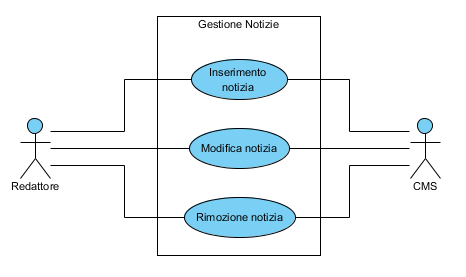
\includegraphics[width=\textwidth]{assets/visualParadigm/GestioneNotizie}
\end{center}
%
%***************  INSERIMENTO NOTIZIA *****************
\cuTab{cu:inserimentoNotizia}
{\getTitletodesc{att:redattore}}
{La persona connessa al sito è autenticata e ha i privilegi di Redattore}
{Nel sistema è presente una nuova notizia}
{\begin{enumCU}
	\item Il caso d'uso ha inizio quando un Redattore richiede di inserire una notizia  
	\item Il sistema richiede di compilare i campi necessari all'inserimento della notizia
	\item Il Redattore inserisce i dati richiesti \label{cuinsnot:2}
	\item Il Redattore conferma i dati richiesti
	\item Il sistema memorizza i dati inseriti e crea una nuova notizia
\end{enumCU}}
%
\cuAlternativo{cu:inserimentoNotizia}
{Flusso alternativo 1}%
{Annulla inserimento}%
{La persona connessa al sito è autenticata e ha i privilegi di Redattore}%
{\postNulle}%
{\begin{enumCU}
		\item Dopo il punto \ref{cuinsnot:2} il Redattore annulla l'inserimento della notizia
	\end{enumCU}}%

\tabcuvspace

%***************  MODIFICA NOTIZIA *****************
\cuTab{cu:modificaNotizia}
{\getTitletodesc{att:redattore}}
{La persona è autenticata e ha i privilegi di Redattore. Nel sistema è presente almeno una notizia}
{Nel sistema è stata modificata una notizia}
{\begin{enumCU}
	\item Il caso d'uso ha inizio quando un Redattore visualizza una notizia, \inc{cu:mostraNotizia}
	\item Il Redattore richiede di modificare la notizia che sta visualizzando
	\item Il sistema richiede di compilarne la scheda associata, precompilata con i dati già presenti nel sistema 
	\item Il Redattore inserisce, modifica o lascia inalterati i dati richiesti \label{cumodnot:2}
	\item Il Redattore conferma i dati richiesti
	\item Il sistema memorizza i dati inseriti e modifica la notizia
\end{enumCU}}
%
\cuAlternativo{cu:modificaNotizia}
{Flusso alternativo 1}%
{Annulla modifica}%
{La persona connessa al sito è autenticata e ha i privilegi di Redattore}%
{\postNulle}%
{\begin{enumCU}
		\item Dopo il punto \ref{cumodnot:2} il Redattore annulla la modifica della notizia
\end{enumCU}}%

\tabcuvspace

%***************  RIMOZIONE NOTIZIA *****************
\cuTab{cu:rimozioneNotizia}
{\getTitletodesc{att:redattore}}
{La persona è autenticata e ha i privilegi di Redattore. Nel sistema è presente almeno una notizia}
{Nel sistema è presente una notizia in meno}
{\begin{enumCU}
	\item Il caso d'uso ha inizio quando un Redattore visualizza una notizia, \inc{cu:mostraNotizia}
	\item Il Redattore richiede di rimuovere la notizia che sta visualizzando
	\item Il sistema chiede conferma della rimozione \label{curemnot:2}
	\item Il Redattore conferma la rimozione
	\item Il sistema rimuove la notizia selezionata
\end{enumCU}}
%
\cuAlternativo{cu:rimozioneNotizia}
{Flusso alternativo 1}%
{Annulla rimozione}%
{La persona è autenticata e ha i privilegi di Redattore. Nel sistema è presente almeno una notizia}%
{\postNulle}%
{\begin{enumCU}
		\item Dopo il punto \ref{curemnot:2} il Redattore annulla la rimozione della notizia
	\end{enumCU}}%

\subsection{Gestione suggerimenti}
\begin{center}
   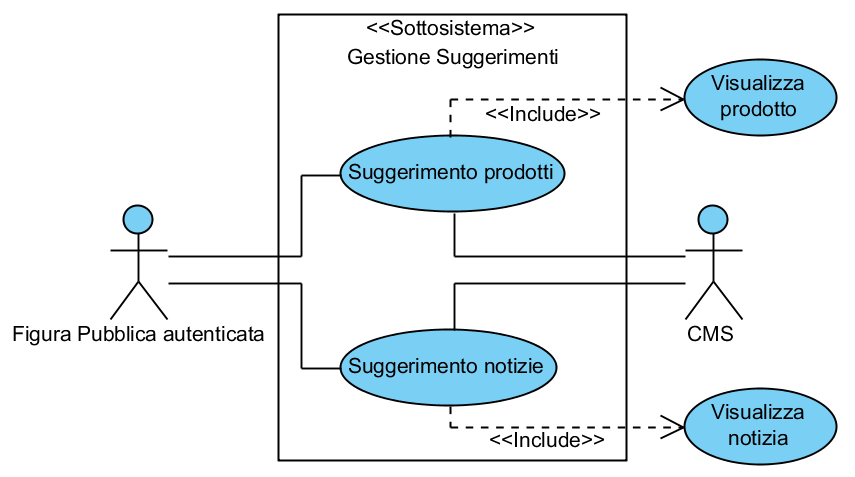
\includegraphics[width=\textwidth]{assets/visualParadigm/GestioneSuggerimenti}
\end{center}
%***************  SUGGERIMENTO PRODOTTI *****************
%Accorpa suggerimento intelligente e simili
\cuTab{cu:suggerimentoProdotti}
{\getTitletodesc{att:figuraPubblicaAutenticata}}
{La persona è autenticata nel sistema ed ha i privilegi di Figura Pubblica Autenticata}
{\postNulle}
{\begin{enumCU}
	\item Il caso d'uso ha inizio quando una Figura Pubblica Autenticata richiede di mostrare prodotti simili al prodotto che sta visualizzando
	\item Il sistema mostra alla Figura Pubblica Autenticata alcuni prodotti simili a quello che sta visualizzando
\end{enumCU}}

\tabcuvspace

%***************  SUGGERIMENTO NOTIZIE *****************
\cuTab{cu:notizieSimili}
{\getTitletodesc{att:figuraPubblicaAutenticata}}
{La persona è autenticata nel sistema ed ha i privilegi di Figura Pubblica Autenticata}
{\postNulle}
{\begin{enumCU}
	\item Il caso d'uso ha inizio quando una Figura Pubblica Autenticata richiede di mostrare notizie simili alla notizia che sta visualizzando
	\item Il sistema mostra alla Figura Pubblica Autenticata alcune notizie simili a quella che sta visualizzando
\end{enumCU}}

\subsection{Gestione account}
\begin{center}
   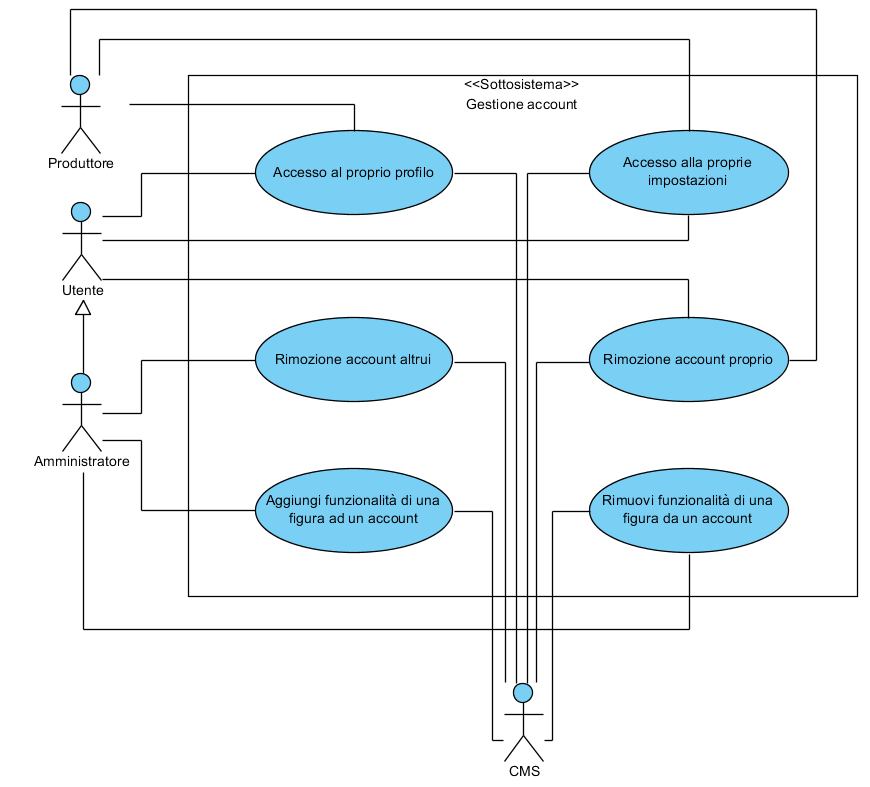
\includegraphics[width=\textwidth]{assets/visualParadigm/GestioneAccount}
\end{center}
%***************  ACCESSO PROFILO *****************
\cuTab{cu:accessoProfilo}
{\getTitletodesc{att:figuraPubblicaAutenticata}, \getTitletodesc{att:figuraAmministrativa}}
{La persona connessa al sito è autenticata}
{\postNulle}
{\begin{enumCU}
	\item Il caso d'uso ha inizio quando una persona autenticata nel sistema richiede di visualizzare il proprio profilo
	\item Il sistema mostra alla persona la pagina del proprio profilo
\end{enumCU}}

\tabcuvspace

%***************  ACCESSO IMPOSTAZIONI *****************
\cuTab{cu:modificaImpostazioni}
{\getTitletodesc{att:figuraPubblicaAutenticata}, \getTitletodesc{att:figuraAmministrativa}}
{La persona connessa al sito è autenticata}
{Le impostazioni della persona sono state modificate}
{\begin{enumCU}
	\item Il caso d'uso ha inizio quando una persona autenticata nel sistema richiede di modificare la pagina delle proprie impostazioni
	\item Il sistema mostra alla persona la pagina delle proprie impostazioni, abilitando solo i campi che la persona può modificare
	\item La persona modifica i campi presenti nella pagina\label{cumodimp:1}
	\item La persona conferma le modifiche effettuate 
	\item Il sistema memorizza le modifiche effettuate
\end{enumCU}}
%
\cuAlternativo{cu:modificaImpostazioni}
{Flusso alternativo 1}%
{Annulla modifica}%
{La persona è autenticata nel sistema}%
{\postNulle}%
{\begin{enumCU}
		\item Dopo il punto \ref{cumodimp:1} annulla le modifiche effettuate
	\end{enumCU}}%

\tabcuvspace

%***************  RIMOZIONE ACCOUNT PROPRIO  *****************
\cuTab{cu:rimozioneAccountProprio}
{\getTitletodesc{att:figuraPubblicaAutenticata}}
{La persona connessa al sito è autenticata ed ha solo i privilegi di Figura Pubblica Autenticata}
{La persona non è più autenticata nel sistema. L'account della persona non è più presente nel sistema}
{\begin{enumCU}
	\item Il caso d'uso ha inizio quando una Figura Pubblica Autenticata nel sistema richiede di rimuovere il proprio account
	\item Il sistema chiede conferma della rimozione dell'account\label{curimaccprop:1}
	\item La persona conferma la rimozione
	\item Il sistema rimuove l'account del richiedente
\end{enumCU}}
%
\cuAlternativo{cu:rimozioneAccountProprio}
{Flusso alternativo 1}%
{Annulla rimozione}%
{La persona connessa al sito è autenticata ed ha solo i privilegi di Figura Pubblica Autenticata}%
{\postNulle}%
{\begin{enumCU}
		\item Dopo il punto \ref{curimaccprop:1} la persona annulla la rimozione dell'account
	\end{enumCU}}%

\tabcuvspace

%***************  RIMOZIONE ACCOUNT ALTRUI  *****************
\cuTab{cu:rimozioneAccountAltrui}
{\getTitletodesc{att:amministratore}}
{La persona è autenticata e ha i privilegi di Amministratore. Nel sistema è presente almeno un altro account}
{Nel sistema è presente account in meno}
{\begin{enumCU}
	\item Il caso d'uso ha inizio quando un Amministratore effettua la ricerca di un profilo, \inc{cu:ricercaProfilo}\label{curimaccaltr:0}
	\item L'Amministratore seleziona un profilo dal risultato della ricerca e richiede al sistema di rimuoverlo 
	\item Il sistema mostra l'account associato al profilo selezionato e chiede conferma della rimozione dell'account\label{curimaccaltr:1}
	\item L'Amministratore conferma la rimozione
	\item Il sistema rimuove l'account selezionato
\end{enumCU}}
%
\cuAlternativo{cu:rimozioneAccountAltrui}
{Flusso alternativo 1}%
{Annulla rimozione}%
{La persona è autenticata e ha i privilegi di Amministratore. Nel sistema è presente almeno un altro account}%
{\postNulle}%
{\begin{enumCU}
	\item Dopo il punto \ref{curimaccaltr:1} l'Amministratore annulla la rimozione dell'account
\end{enumCU}}%
%	
\cuAlternativo{cu:rimozioneAccountAltrui}
{Flusso alternativo 2}%
{Annulla operazione di selezione}%
{La persona è autenticata e ha i privilegi di Amministratore. Nel sistema è presente almeno un altro account}%
{\postNulle}%
{\begin{enumCU}
	\item Dopo il punto \ref{curimaccaltr:0} l'Assistente annulla la selezione
\end{enumCU}}%

\tabcuvspace

%***************  Modifica privilegi  *****************
\cuTab{cu:modificaPrivilegiAccount}
{\getTitletodesc{att:amministratore}}
{La persona è autenticata e ha i privilegi di Amministratore. Nel sistema è presente almeno un account}
{Sono stati aggiornati i privilegi di un account}
{\begin{enumCU}
	\item Il caso d'uso ha inizio quando un Amministratore effettua la ricerca di un profilo, \inc{cu:ricercaProfilo}\label{cufornpriv:0}
	\item L'Amministratore seleziona un profilo dal risultato della ricerca
	\item Il sistema mostra all'Amministratore la lista dei privilegi, specificando quelli posseduti dall'account associato al profilo selezionato
	\item Il sistema chiede di modificare i privilegi posseduti dall'account
	\item L'Amministratore seleziona quali privilegi vuole fornire all'account\label{cufornpriv:1}
	\item L'Amministratore conferma la selezione
	\item Il sistema memorizza le scelte effettuate
\end{enumCU}}
%
\cuAlternativo{cu:modificaPrivilegiAccount}
{Flusso alternativo 1}%
{Annulla operazione}%
{La persona è autenticata e ha i privilegi di Amministratore. Nel sistema è presente almeno un account}%
{\postNulle}%
{\begin{enumCU}
		\item Dopo il punto \ref{cufornpriv:1} l'Amministratore annulla l'operazione
	\end{enumCU}}%
%	
\cuAlternativo{cu:modificaPrivilegiAccount}
{Flusso alternativo 2}%
{Annulla operazione di selezione}%
{La persona è autenticata e ha i privilegi di Amministratore. Nel sistema è presente almeno un account}%
{\postNulle}%
{\begin{enumCU}
		\item Dopo il punto \ref{cufornpriv:0} l'Assistente annulla la selezione
\end{enumCU}}%

\tabcuvspace

%***************  Aggiungi privilegi  *****************
%\cuTab{cu:aggiungiPrivilegiAccount}
%{\getTitletodesc{att:amministratore}}
%{La persona è autenticata e ha i privilegi di Amministratore. Nel sistema è presente almeno un account}
%{L'account da modificare ha i privilegi della figura scelta, oltre a quelli già posseduti}
%{\begin{enumCU}
%	\item Il caso d'uso ha inizio quando un Amministratore vuole fornire un ulteriore privilegio ad un account
%	\item Il sistema chiede quali privilegi fornire all'account 
%	\item L'Amministratore seleziona quale privilegio si vuole fornire all'account \label{cufornpriv:1}
%	\item L'Amministratore conferma la selezione
%	\item Il sistema accetta la selezione effettuata
%\end{enumCU}}
%%
%\cuAlternativo{cu:aggiungiPrivilegiAccount}
%{Flusso alternativo 1}%
%{Annulla operazione}%
%{La persona è autenticata e ha i privilegi di Amministratore. L'account da modificare è presente nel sistema e non ha già i privilegi della figura scelta}%
%{\postNulle}%
%{\begin{enumCU}
%		\item Dopo il punto \ref{cufornpriv:1} l'Amministratore annulla l'operazione
%	\end{enumCU}}%
%
%\tabcuvspace
%
%***************  Rimuovi privilegi  *****************
%\cuTab{cu:rimuoviPrivilegiAccount}
%{\getTitletodesc{att:amministratore}}
%{La persona è autenticata e ha i privilegi di Amministratore. L'account da modificare è presente nel sistema e ha già i privilegi della figura scelta}
%{L'account da modificare non ha più i privilegi della figura scelta, ma mantiene gli altri}
%{\begin{enumCU}
%	\item Il caso d'uso ha inizio quando un Amministratore vuole rimuovere un privilegio ad un account%
%	\item Il sistema chiede quali privilegi rimuovere dall'account  fra quelli che possiede
%	\item L'Amministratore seleziona quale privilegio si vuole rimuovere dall'account \label{curimpriv:1}
%	\item L'Amministratore conferma la selezione
%	\item Il sistema accetta la selezione effettuata
%\end{enumCU}}
%
%\cuAlternativo{cu:rimuoviPrivilegiAccount}
%{Flusso alternativo 1}%
%{Annulla operazione}%
%{La persona è autenticata e ha i privilegi di Amministratore. L'account da modificare è presente nel sistema e ha già i privilegi della figura scelta}%
%{\postNulle}%
%{\begin{enumCU}%
%		\item Dopo il punto \ref{curimpriv:1} l'Amministratore annulla l'operazione%
%	\end{enumCU}}%


%***************  Gestione valutazioni *****************
\subsection{Gestione valutazioni}
\begin{center}
   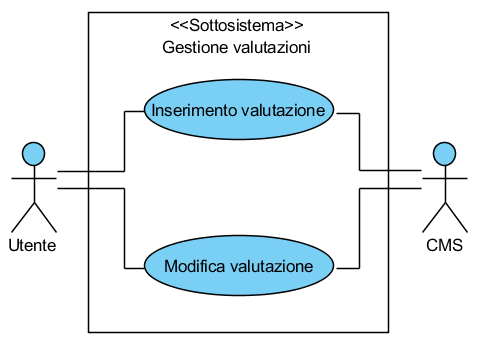
\includegraphics[width=\textwidth]{assets/visualParadigm/GestioneValutazioni}
\end{center}
\cuTab{cu:inserisciValutazioneProdotto}
{\getTitletodesc{att:utente}}
{La persona è autenticata e ha i privilegi di Utente. Nel sistema è presente almeno un prodotto che non è già stato valutato dalla persona}
{Nel sistema è stata aggiunta la valutazione della persona per un prodotto}
{\begin{enumCU}
	\item Il caso d'uso ha inizio quando un Utente visualizza un prodotto, \inc{cu:mostraProdotto}
	\item L'Utente richiede di effettuare la valutazione del prodotto che sta visualizzando
	\item Il sistema richiede all'Utente la valutazione per quel prodotto
	\item L'Utente inserisce la valutazione
	\item Il sistema memorizza la valutazione
\end{enumCU}}

\tabcuvspace

\cuTab{cu:modificaValutazioneProdotto}
{\getTitletodesc{att:utente}}
{La persona è autenticata, ha i privilegi di Utente e ha effettuato una valutazione di un prodotto presente nel sistema}
{Nel sistema è stata modificata la valutazione di un prodotto inserita da una persona}
{\begin{enumCU}
	\item Il caso d'uso ha inizio quando un Utente visualizza un prodotto che ha già valutato, \inc{cu:mostraProdotto}
	\item L'Utente richiede di modificare la valutazione del prodotto
	\item Il sistema mostra all'Utente la valutazione che ha effettuato per quel prodotto
	\item L'Utente inserisce la nuova valutazione
	\item Il sistema memorizza la nuova valutazione inserita
\end{enumCU}}

%***************  Gestione recensione *****************
\subsection{Gestione recensioni}
\begin{center}
   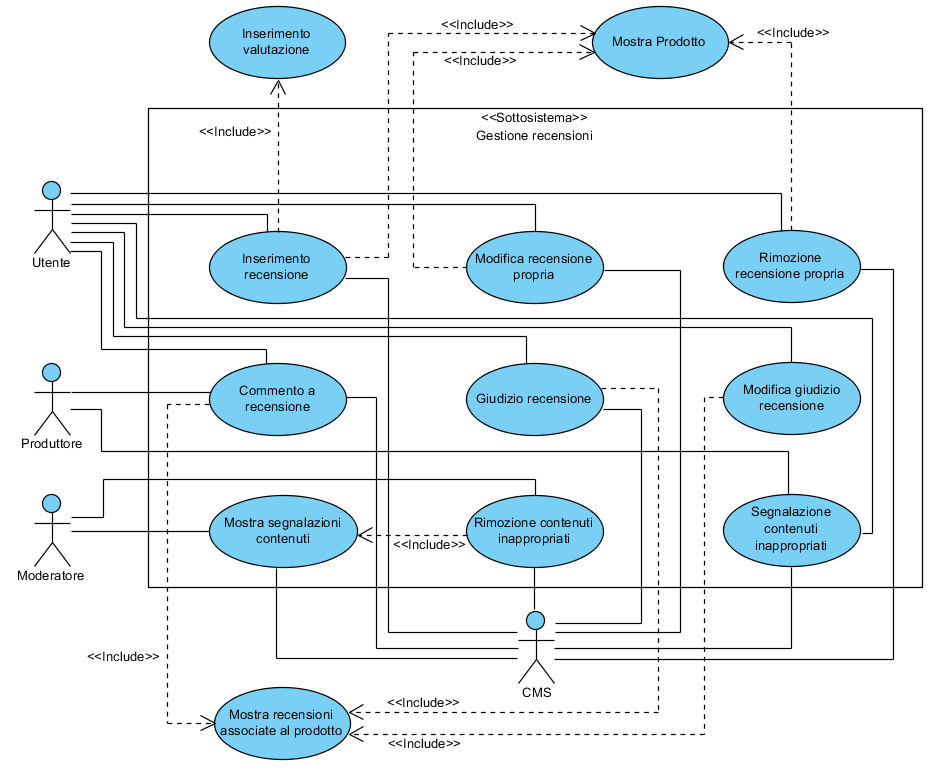
\includegraphics[width=\textwidth]{assets/visualParadigm/GestioneRecensioni}
\end{center}
\cuTab{cu:inserisciRecensioneProdotto}
{\getTitletodesc{att:utente}}
{La persona è autenticata come Utente. Il prodotto è presente nel sistema e non è già stato recensito dall'Utente}
{La recensione dell'Utente per quel prodotto è aggiunta nel sistema}
{\begin{enumCU}
	\item Il caso d'uso ha inizio quando un Utente richiede di effettuare la recensione di un prodotto presente nel sistema
	\item Il sistema richiede all'Utente il testo da inserire come recensione
	\item L'Utente inserisce la recensione \label{addrec:3}
	\item L'Utente conferma la recensione inserita
	\item Il sistema accetta la recensione
\end{enumCU}}
%
\cuAlternativo{cu:inserisciRecensioneProdotto}
{Flusso alternativo 1}%
{Annulla inserimento}%
{La persona è autenticata come Utente. Il prodotto è presente nel sistema e non è già stato recensito dall'Utente}%
{\postNulle}%
{\begin{enumCU}
		\item Dopo il punto \ref{addrec:3}, l'Utente annulla l'operazione di inserimento
	\end{enumCU}}%

\tabcuvspace

\cuTab{cu:modificaRecensioneProdotto}
{\getTitletodesc{att:utente}}
{La persona è autenticata come Utente e ha effettuato una recensione di un prodotto presente nel sistema}
{La recensione viene modificata correttamente}
{\begin{enumCU}
	\item Il caso d'uso ha inizio quando un Utente richiede di modificare una sua recensione di un prodotto presente nel sistema
	\item Il sistema mostra all'Utente la recensione che ha effettuato per quel prodotto
	\item L'Utente inserisce la nuova recensione \label{newrec:3}
	\item L'Utente conferma la nuova recensione inserita
	\item Il sistema accetta la nuova recensione
\end{enumCU}}
%
\cuAlternativo{cu:modificaRecensioneProdotto}
{Flusso alternativo 1}%
{Annulla modifiche}%
{La persona è autenticata come Utente e ha effettuato una recensione di un prodotto presente nel sistema}
{\postNulle}%
{\begin{enumCU}
		\item Dopo il punto \ref{newrec:3}, l'Utente annulla l'operazione di modifica
	\end{enumCU}}%

\tabcuvspace

\cuTab{cu:eliminaRecensioneProdotto}
{\getTitletodesc{att:utente}}
{La persona è autenticata come Utente e ha effettuato una recensione di un prodotto presente nel sistema}
{La recensione viene rimossa dal sistema correttamente }
{\begin{enumCU}
	\item Il caso d'uso ha inizio quando un Utente richiede di rimuovere una sua recensione di un prodotto presente nel sistema
	\item Il sistema mostra all'Utente la recensione che ha effettuato per quel prodotto
	\item Il sistema richiede di confermare la rimozione \label{remrec:3}
	\item L'Utente conferma la rimozione
	\item Il sistema rimuove la recensione
\end{enumCU}}
%
\cuAlternativo{cu:eliminaRecensioneProdotto}
{Flusso alternativo 1}%
{Annulla rimozione}%
{La persona è autenticata come Utente e ha effettuato una recensione di un prodotto presente nel sistema}
{\postNulle}%
{\begin{enumCU}
		\item Dopo il punto \ref{remrec:3}, l'Utente annulla l'operazione di rimozione
	\end{enumCU}}%

\tabcuvspace

\cuTab{cu:commentoRecensione}
{\getTitletodesc{att:utente}, \getTitletodesc{att:produttore}}
{La persona è autenticata come Utente o come Produttore. La recensione di un prodotto è presente nel sistema}
{Il commento viene aggiunto ai commenti di quella recensione}
{\begin{enumCU}
	\item Il caso d'uso ha inizio quando una persona, autenticata come Utente o come Produttore, richiede di effettuare un commento ad una recensione di un prodotto presente nel sistema
	\item Il sistema mostra alla persona la recensione
	\item Il sistema richiede di inserire il commento 
	\item La persona inserisce il commento \label{addcom:3}
	\item La persona conferma il commento inserito
	\item Il sistema accetta il commento
\end{enumCU}}
%
\cuAlternativo{cu:commentoRecensione}
{Flusso alternativo 1}%
{Annulla rimozione}%
{La persona è autenticata come Utente o come Produttore. La recensione di un prodotto è presente nel sistema}
{\postNulle}%
{\begin{enumCU}
		\item Dopo il punto \ref{addcom:3}, la persona, autenticata come Utente o come Produttore, annulla l'operazione di inserimento
	\end{enumCU}}%

\tabcuvspace

\cuTab{cu:giudizioRecensione}
{\getTitletodesc{att:utente}}{La persona è autenticata come Utente. La recensione di un prodotto è presente nel sistema}
{Il giudizio per quella recensione di quell'Utente è presente nel sistema}
{\begin{enumCU}
	\item Il caso d'uso ha inizio quando un Utente richiede di esprimere un giudizio (positivo o negativo) su una recensione di un prodotto presente nel sistema
	\item Il sistema mostra all'Utente la recensione
	\item Il sistema richiede all'Utente il giudizio per quella recensione
	\item L'Utente inserisce il giudizio
	\item Il sistema accetta il giudizio
\end{enumCU}}


\cuTab{cu:modificaGiudizioRecensione}
{\getTitletodesc{att:utente}}
{La persona è autenticata come Utente. La recensione di un prodotto è presente nel sistema}
{Il giudizio per quella recensione viene modificato correttamente}
{\begin{enumCU}
	\item Il caso d'uso ha inizio quando un Utente richiede di modificare un giudizio di una recensione di un prodotto presente nel sistema
	\item Il sistema mostra all'Utente il suo giudizio per quella recensione
	\item Il sistema richiede all'Utente il nuovo giudizio per quella recensione
	\item L'Utente inserisce il nuovo giudizio
	\item Il sistema accetta il nuovo giudizio
\end{enumCU}}

\tabcuvspace

\cuTab{cu:segnalazioneContenutiInap}
{\getTitletodesc{att:utente}, \getTitletodesc{att:produttore}}
{La persona è autenticata come Utente o come Produttore. Il contenuto è presente nel sistema}
{La segnalazione viene memorizzata nel sistema}
{\begin{enumCU}
	\item Il caso d'uso ha inizio quando una persona, autenticata come Utente o come Produttore, richiede di segnalare un contenuto inappropriato presente nel sistema
	\item Il sistema richiede alla persona di specificare il motivo della segnalazione
	\item La persona inserisce il motivo della segnalazione
	\item Il sistema accetta la segnalazione
\end{enumCU}}

\tabcuvspace

\cuTab{cu:mostraSegnContenutiInap}
{\getTitletodesc{att:moderatore}}
{La persona è autenticata ed ha i privilegi di Moderatore. La segnalazione è presente nel sistema}
{La segnalazione è stata gestita dal Moderatore}
{\begin{enumCU}
	\item Il caso d'uso ha inizio quando una Moderatore richiede di visualizzare una segnalazione
	\item Il sistema mostra al Moderatore la segnalazione \label{delsegn:3}
\end{enumCU}}
%
\cuAlternativo{cu:mostraSegnContenutiInap}
{Flusso alternativo 1}%
{Elimina segnalazione}%
{La persona è autenticata ed ha i privilegi Moderatore. La segnalazione è presente nel sistema}
{La segnalazione non è più presente nel sistema}%
{\begin{enumCU}
		\item Dopo il punto \ref{delsegn:3}, il Moderatore elimina la segnalazione
\end{enumCU}}%
%marcare segfnalazione come risolta/eliminarla dalla lista

\tabcuvspace

\cuTab{cu:rimozioneContenutiInap}
{\getTitletodesc{att:moderatore}}
{La persona è autenticata ed ha i privilegi Moderatore. Il contenuto da rimuovere è presente nel sistema}
{Il contenuto da rimuovere non è più presente nel sistema}
{\begin{enumCU}
	\item Il caso d'uso ha inizio quando un Moderatore richiede di rimuovere un contenuto inappropriato presente nel sistema
	\item Il sistema richiede al Moderatore di confermare la rimozione
	\item Il Moderatore conferma la rimozione \label{delcont:3}
	\item Il sistema rimuove il contenuto inappropriato
\end{enumCU}}
%
\cuAlternativo{cu:rimozioneContenutiInap}
{Flusso alternativo 1}%
{Annulla rimozione}%
{La persona è autenticata ed ha i privilegi Moderatore. Il contenuto da rimuovere è presente nel sistema}
{\postNulle}%
{\begin{enumCU}
		\item Dopo il punto \ref{delcont:3}, il Moderatore annulla l'operazione di rimozione
\end{enumCU}}%


\subsection{Interazione tra figure}
\begin{center}
   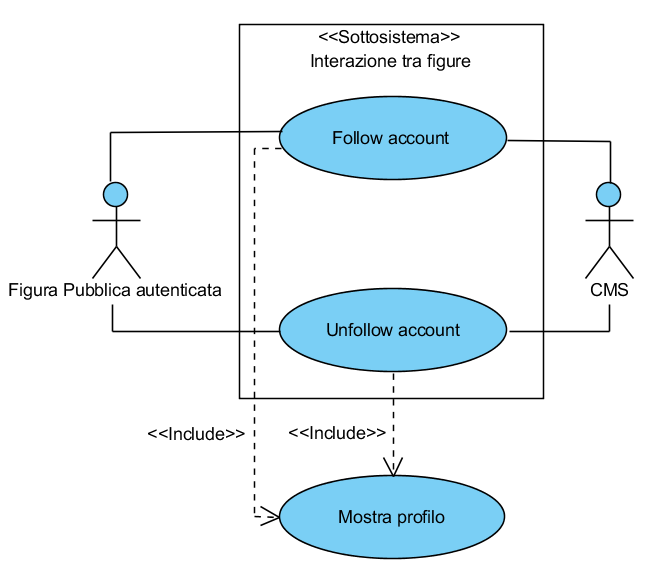
\includegraphics[width=\textwidth]{assets/visualParadigm/InterazioneTraFigure}
\end{center}
%****************** FOLLOW ACCOUNT ***********
\cuTab{cu:followAccount}
{\getTitletodesc{att:utente}, \getTitletodesc{att:produttore}}
{La persona è autenticata come Utente o come Produttore. L'account da seguire è presente nel sistema}
{L'account da seguire viene aggiunto alla lista degli account che la persona segue}
{\begin{enumCU}
	\item Il caso d'uso ha inizio quando un Utente o un Produttore richiede di seguire un altro account per riceverne gli aggiornamenti
	\item Il sistema accetta l`operazione
\end{enumCU}}

\tabcuvspace

%****************** UNFOLLOW ACCOUNT ***********
\cuTab{cu:unFollowAccount}
{\getTitletodesc{att:utente}, \getTitletodesc{att:produttore}}
{La persona è autenticata come Utente o come Produttore. L'account seguito è presente nel sistema}
{L'account seguito viene rimosso dalla lista degli account che la persona segue}
{\begin{enumCU}
	\item Il caso d'uso ha inizio quando un Utente o un Produttore richiede di smettere di seguire un altro account che già segue
	\item Il sistema accetta l`operazione
\end{enumCU}}

\subsection{Gestione ticket}
\begin{center}
   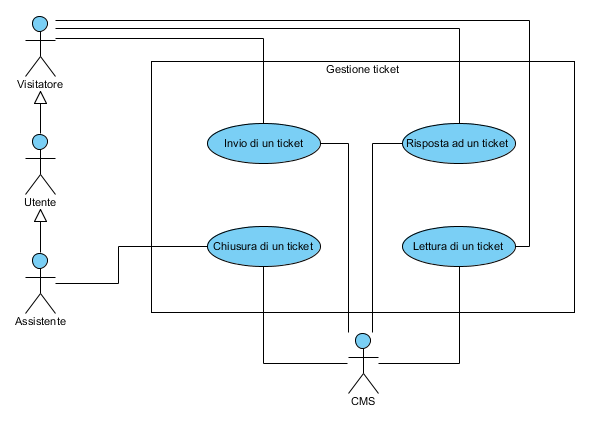
\includegraphics[width=\textwidth]{assets/visualParadigm/GestioneTicket}
\end{center}
%****************** INVIO TICKET ***********
\cuTab{cu:ticketInvio}
{\getTitletodesc{att:utente}, \getTitletodesc{att:produttore}}
{La persona è autenticata come Utente o come Produttore}
{Viene creato un nuovo ticket}
{\begin{enumCU}
	\item Il caso d'uso ha inizio quando un Utente o un Produttore richiedono la creazione di un ticket per ricevere assistenza
	\item Il sistema richiede di compilare la scheda necessaria alla creazione del ticket
	\item La persona compila la scheda \label{cucretick:1}
	\item La persona conferma i dati inseriti
	\item Il sistema accetta la creazione del ticket
\end{enumCU}}
%
\cuAlternativo{cu:ticketInvio}
{Flusso alternativo 1}%
{Annulla creazione ticket}%
{La persona è autenticata come Utente o come Produttore}%
{\postNulle}%
{\begin{enumCU}
		\item Dopo il punto \ref{cucretick:1} l'Utente (o il produttore) annulla la creazione del ticket
	\end{enumCU}}%

\tabcuvspace

%****************** RISPOSTA TICKET ***********
\cuTab{cu:ticketRisposta}
{\getTitletodesc{att:utente}, \getTitletodesc{att:produttore}, \getTitletodesc{att:assistente}}
{La persona è autenticata come Utente o come Produttore e il ticket è stato creato da quella persona, oppure ha i privilegi di Assistente}
{La risposta al ticket è aggiunta nel sistema}
{\begin{enumCU}
	\item Il caso d'uso ha inizio quando il creatore di un ticket o un Assistente richiedono di inserire una risposta ad un ticket
	\item Il sistema richiede di compilare la scheda necessaria alla creazione della risposta
	\item Colui che intende inserire la risposta compila la scheda necessaria all'inserimento della risposta\label{curisptick:1}
	\item Colui che intende inserire la risposta conferma i dati inseriti
	\item Il sistema accetta la creazione della risposta al ticket
\end{enumCU}}
%
\cuAlternativo{cu:ticketRisposta}
{Flusso alternativo 1}%
{Annulla risposta ticket}%
{La persona è autenticata come Utente o come Produttore e il ticket è stato creato da quella persona, oppure ha i privilegi di Assistente}%
{\postNulle}%
{\begin{enumCU}
		\item Dopo il punto \ref{curisptick:1} colui che intende inserire la risposta annulla l'inserimento
	\end{enumCU}}%

\tabcuvspace

%****************** CHIUDI TICKET ***********
\cuTab{cu:ticketChiudi}
{\getTitletodesc{att:utente}, \getTitletodesc{att:produttore}, \getTitletodesc{att:assistente}}
{La persona è autenticata come Utente o come Produttore e il ticket è stato creato da quella persona, oppure ha i privilegi di Assistente}
{Il ticket viene etichettato come chiuso}
{\begin{enumCU}
	\item Il caso d'uso ha inizio quando il creatore del ticket o un Assistente richiede di chiudere il ticket
	\item Il sistema richiede conferma della chiusura \label{cuchiutick:1}
	\item La persona conferma la chiusura del ticket
	\item Il sistema accetta l'operazione
\end{enumCU}}
%
\cuAlternativo{cu:ticketChiudi}
{Flusso alternativo 1}%
{Annulla chiusura ticket}%
{La persona è autenticata come Utente o come Produttore e il ticket è stato creato da quella persona, oppure ha i privilegi di Assistente}%
{\postNulle}%
{\begin{enumCU}
		\item Dopo il punto \ref{cuchiutick:1} colui che intende inserire la risposta annulla l'inserimento
	\end{enumCU}}%

\tabcuvspace

%****************** LEGGI TICKET ***********
\cuTab{cu:ticketLettura}
{\getTitletodesc{att:utente}, \getTitletodesc{att:produttore}, \getTitletodesc{att:assistente}}
{La persona è autenticata come Utente o come Produttore e il ticket è stato creato da quella persona, oppure ha i privilegi di Assistente}
{Il ticket viene visualizzato}
{\begin{enumCU}
	\item Il caso d'uso ha inizio quando il creatore di un ticket o un Assistente richiedono di visualizzare un ticket
	\item Il sistema mostra il ticket al richiedente
\end{enumCU}}


\subsection{Ricerca contenuti}
\begin{center}
   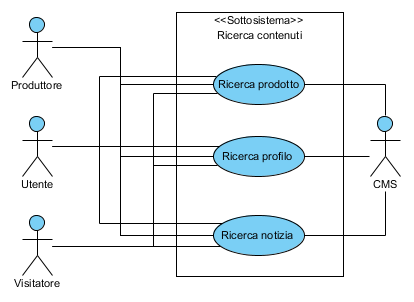
\includegraphics[width=\textwidth]{assets/visualParadigm/RicercaContenuti}
\end{center}
%****************** RICERCA PRODOTTO ***********
\cuTab{cu:ricercaProdotto}
{\getTitletodesc{att:visitatore}, \getTitletodesc{att:utente}, \getTitletodesc{att:produttore}}
{La persona è connessa al sito}
{I risultati della ricerca sono visualizzati}
{\begin{enumCU}
	\item Il caso d'uso ha inizio quando la persona richiede di effettuare una ricerca di un prodotto
	\item Il sistema richiede di complilare la scheda necessaria per definire i parametri di ricerca
	\item La persona inserisce i dati negli appositi campi \label{curicprod:1}
	\item La persona conferma i dati inseriti
	\item Il sistema effettua la ricerca richiesta
\end{enumCU}}
%
\cuAlternativo{cu:ricercaProdotto}
{Flusso alternativo 1}%
{Annulla ricerca}%
{La persona è connessa al sito}%
{\postNulle}%
{\begin{enumCU}
		\item Dopo il punto \ref{curicprod:1} la persona annulla la ricerca
	\end{enumCU}}%

\tabcuvspace

%\cuTab{cu:selezionaProdotto}
%{\getTitletodesc{att:visitatore}, \getTitletodesc{att:utente}, \getTitletodesc{att:produttore}}
%{La persona è connessa al sito}
%{I risultati della ricerca sono visualizzati}
%{\begin{enumCU}
%	\item Il caso d'uso ha inizio quando la persona richiede di effettuare una ricerca di un prodotto
%	\item Il sistema richiede di complilare la scheda necessaria per definire i parametri di ricerca
%	\item La persona inserisce i dati negli appositi campi \label{curicprod:1}
%	\item La persona conferma i dati inseriti
%	\item Il sistema effettua la ricerca richiesta
%\end{enumCU}}
%
%\tabcuvspace

%****************** RICERCA PROFILO ***********
\cuTab{cu:ricercaProfilo}
{\getTitletodesc{att:visitatore}, \getTitletodesc{att:utente}, \getTitletodesc{att:produttore}}
{La persona è connessa al sito}
{I risultati della ricerca sono visualizzati}
{\begin{enumCU}
	\item Il caso d'uso ha inizio quando la persona richiede di effettuare una ricerca di un profilo
	\item Il sistema richiede di complilare la scheda necessaria per definire i parametri di ricerca
	\item La persona inserisce i dati negli appositi campi \label{curicprof:1}
	\item La persona conferma i dati inseriti
	\item Il sistema effettua la ricerca richiesta
\end{enumCU}}
%
\cuAlternativo{cu:ricercaProfilo}
{Flusso alternativo 1}%
{Annulla ricerca}%
{La persona è connessa al sito}%
{\postNulle}%
{\begin{enumCU}
		\item Dopo il punto \ref{curicprof:1} la persona annulla la ricerca
	\end{enumCU}}%

\tabcuvspace

%\cuTab{cu:selezionaProfilo}
%{\getTitletodesc{att:visitatore}, \getTitletodesc{att:utente}, \getTitletodesc{att:produttore}}
%{La persona è connessa al sito}
%{I risultati della ricerca sono visualizzati}
%{\begin{enumCU}
%	%\item Il caso d'uso ha inizio quando la persona richiede di effettuare una ricerca di un profilo
%	%\item Il sistema richiede di complilare la scheda necessaria per definire i parametri di ricerca
%	\item La persona inserisce i dati negli appositi campi \label{curicprof:1}
%	\item La persona conferma i dati inseriti
%	\item Il sistema effettua la ricerca richiesta
%\end{enumCU}}
%
%\tabcuvspace

%****************** RICERCA NOTIZIA ***********
\cuTab{cu:ricercaNotizia}
{\getTitletodesc{att:visitatore}, \getTitletodesc{att:utente}, \getTitletodesc{att:produttore}}
{La persona è connessa al sito}
{I risultati della ricerca sono visualizzati}
{\begin{enumCU}
	\item Il caso d'uso ha inizio quando la persona richiede di effettuare una ricerca di una notizia
	\item Il sistema richiede di compilare la scheda necessaria per definire i parametri di ricerca
	\item La persona inserisce i dati negli appositi campi \label{curicnot:1}
	\item La persona conferma i dati inseriti
	\item Il sistema effettua la ricerca richiesta
\end{enumCU}}
%
\cuAlternativo{cu:ricercaNotizia}
{Flusso alternativo 1}%
{Annulla ricerca}%
{La persona è connessa al sito}%
{\postNulle}%
{\begin{enumCU}
		\item Dopo il punto \ref{curicnot:1} la persona annulla la ricerca
	\end{enumCU}}%

%\tabcuvspace
%
%\cuTab{cu:selezionaNotizia}
%{\getTitletodesc{att:visitatore}, \getTitletodesc{att:utente}, \getTitletodesc{att:produttore}}
%{La persona è connessa al sito}
%{I risultati della ricerca sono visualizzati}
%{\begin{enumCU}
%	%\item Il caso d'uso ha inizio quando la persona richiede di effettuare una ricerca di una notizia
%	%\item Il sistema richiede di compilare la scheda necessaria per definire i parametri di ricerca
	%\item La persona inserisce i dati negli appositi campi \label{curicnot:1}
	%\item La persona conferma i dati inseriti
	%\item Il sistema effettua la ricerca richiesta
%\end{enumCU}}

\subsection{Gestione prodotti mancanti}
\begin{center}
   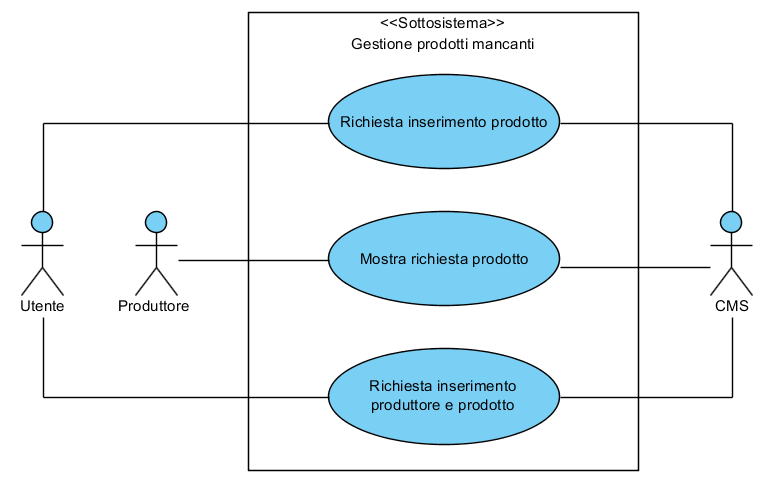
\includegraphics[width=\textwidth]{assets/visualParadigm/GestioneProdottiMancanti}
\end{center}
%****************** RICHIESTA PRODOTTO ***********
\cuTab{cu:richiestaInsProdotto}
{\getTitletodesc{att:utente}}
{La persona è autenticata come Utente. Il Produttore è presente nel sistema. Il prodotto non è presente nel sistema}
{La richiesta è inviata al Produttore}
{\begin{enumCU}
		\item Il caso d'uso ha inizio quando un Utente richiede ad un Produttore di inserire un suo prodotto mancante
		\item Il sistema richiede di compilare una scheda provvisoria del prodotto da inserire
		\item L'Utente inserisce i dati richiesti \label{curicinsimmpro:1}
		\item L'Utente conferma i dati inseriti 
		\item Il sistema richiede zero o più percorsi nel file system, o nella rete, delle immagini del prodotto da inserire
		\item L'Utente inserisce nell'apposito campo zero o più percorsi delle immagini che vuole inserire \label{curicinsimmpro:2}
		\item L'Utente conferma i percorsi inseriti \label{curicinsimmpro:3}
		\item Il sistema accetta i dati inseriti, i percorsi inseriti e salva le immagini nel sistema
	\end{enumCU}}
%
\cuAlternativo{cu:richiestaInsProdotto}
{Flusso alternativo 1}%
{Annulla richiesta}%
{La persona è autenticata come Utente. Il Produttore è presente nel sistema. Il prodotto non è presente nel sistema}%
{\postNulle}%
{\begin{enumCU}
		\item Dopo il punto \ref{curicinsimmpro:2} o dopo il punto \ref{curicinsimmpro:1} l'Utente annulla la richiesta
	\end{enumCU}}%
%
\cuAlternativo{cu:richiestaInsProdotto}
{Flusso alternativo 2}%
{Errore richiesta}%
{La persona è autenticata come Utente. Il Produttore è presente nel sistema. Il prodotto non è presente nel sistema}%
{\postNulle}%
{\begin{enumCU}
		\item Dopo il punto \ref{curicinsimmpro:3} il sistema non riesce a trovare, caricare o inserire correttamente una o più immagini
	\end{enumCU}}%

\tabcuvspace

\cuTab{cu:mostraRichiestaInsProdotto}
{\getTitletodesc{att:produttore}}
{La persona è autenticata come Produttore. Nel sistema è presente una richiesta di inserimento prodotto a lui indirizzata}
{Il prodotto suggerito è presente nella vetrina del Produttore}
{\begin{enumCU}
		\item Il caso d'uso ha inizio quando un Produttore richiedere di visualizzare le proprie richieste di aggiunta di prodotti in sospeso
		\item Il sistema richiede di selezionare quale richiesta visualizzare
		\item Il Produttore seleziona quale richiesta visualizzare
		\item Il sistema mostra al Produttore la scheda provvisoria del prodotto compilata dall'Utente che ha effettuato la richiesta \label{cuvisricprodel}
		\item Il Produttore modifica i campi nella scheda o inserisce quelli mancanti \label{cuvisricpro:1}
		\item Il Produttore conferma i dati inseriti
		\item Il sistema richiede zero o più percorsi nel file system, o nella rete, delle immagini del prodotto da inserire
		\item Il Produttore inserisce nell'apposito campo uno (zero se già inserite dall'utente) o più percorsi delle immagini che vuole inserire \label{cuvisricpro:2}
		\item Il Produttore conferma i percorsi inseriti \label{cuvisricpro:3}
		\item Il sistema accetta i dati inseriti, i percorsi inseriti e salva le immagini nel sistema
	\end{enumCU}}
%
\cuAlternativo{cu:mostraRichiestaInsProdotto}
{Flusso alternativo 1}%
{Elimina richiesta}%
{La persona è autenticata come Produttore. Nel sistema è presente una richiesta di inserimento prodotto a lui indirizzata}
{La richiesta non è più presente nel sistema}%
{\begin{enumCU}
		\item Dopo il punto \ref{cuvisricprodel} il Produttore richede di eliminare la richiesta
		\item Il sistema accetta l'operazione
	\end{enumCU}}%
%
\cuAlternativo{cu:mostraRichiestaInsProdotto}
{Flusso alternativo 2}%
{Annulla inserimento}%
{La persona è autenticata come Produttore. Nel sistema è presente una richiesta di inserimento prodotto a lui indirizzata}
{\postNulle}%
{\begin{enumCU}
		\item Dopo il punto \ref{cuvisricpro:2} o dopo il punto \ref{cuvisricpro:1} il Produttore annulla l'inserimento
	\end{enumCU}}%
%
\cuAlternativo{cu:mostraRichiestaInsProdotto}
{Flusso alternativo 3}%
{Errore inserimento}%
{La persona è autenticata come Produttore. Nel sistema è presente una richiesta di inserimento prodotto a lui indirizzata}
{\postNulle}%
{\begin{enumCU}
		\item Dopo il punto \ref{cuvisricpro:3} il sistema non riesce a trovare, caricare o inserire correttamente una o più immagini
	\end{enumCU}}%

\tabcuvspace

\cuTab{cu:richiestaInsProduttore}
{\getTitletodesc{att:utente}}
{La persona è autenticata come Utente. Il Produttore non è presente nel sistema}
{Nel sistema è presente un ticket riguardante la richiesta}
{\begin{enumCU}
		\item Il caso d'uso ha inizio quando un Utente richiedere di inserire un prodotto mancante di un Produttore non presente nel sistema
		\item Il sistema richiede di compilare una scheda provvisoria del prodotto da inserire
		\item L'Utente inserisce i dati richiesti \label{cuinsproduttore:1}
		\item L'Utente conferma i dati inseriti 
		\item Il sistema richiede zero o più percorsi nel file system, o nella rete, delle immagini del prodotto da inserire
		\item L'Utente inserisce nell'apposito campo zero o più percorsi delle immagini che vuole inserire \label{cuinsproduttore:2}
		\item L'Utente conferma i percorsi inseriti \label{cuinsproduttore:3}
		\item Il sistema accetta i dati inseriti, i percorsi inseriti e salva le immagini nel sistema
		\item Il sistema richiede di compilare un profilo provvisorio, con almeno un nome e un recapito, del produttore
		\item L'Utente inserisce i dati richiesti \label{cuinsproduttore:0}
		\item L'Utente conferma i dati inseriti
		\item Il sistema accetta i dati inseriti
	\end{enumCU}}
%
\cuAlternativo{cu:richiestaInsProduttore}
{Flusso alternativo 1}%
{Annulla inserimento}%
{La persona è autenticata come Utente. Il Produttore non è presente nel sistema}%
{\postNulle}%
{\begin{enumCU}
		\item Dopo il punto \ref{cuinsproduttore:1}, il punto \ref{cuinsproduttore:2} o dopo il punto \ref{cuinsproduttore:0} l'Utente annulla l'operazione
	\end{enumCU}}%
%
\cuAlternativo{cu:richiestaInsProduttore}
{Flusso alternativo 2}%
{Errore inserimento}%
{La persona è autenticata come Utente. Il Produttore non è presente nel sistema}%
{\postNulle}%
{\begin{enumCU}
		\item Dopo il punto \ref{cuinsproduttore:3} il sistema non riesce a trovare, caricare o inserire correttamente una o più immagini
	\end{enumCU}}%



\subsection{Visualizzazione contenuti pubblici}
\begin{center}
   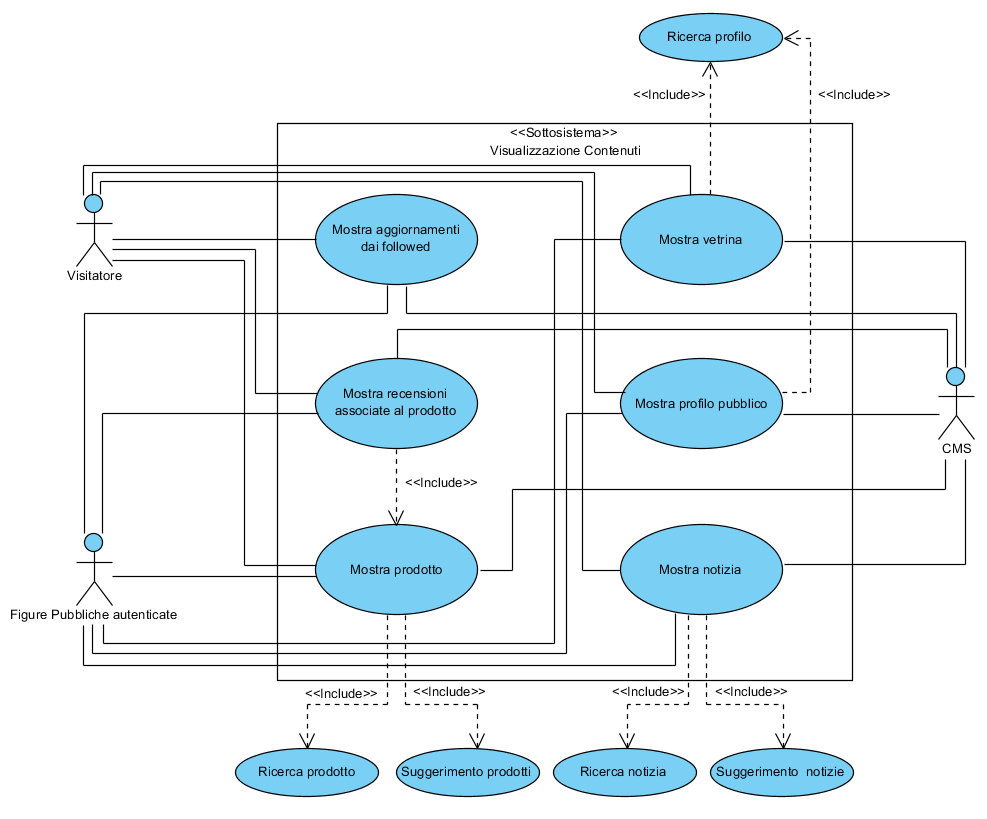
\includegraphics[width=\textwidth]{assets/visualParadigm/Visualizzazione}
\end{center}
%accorpa visalizza prodotti in vetrina e visualizza vetrina
\cuTab{cu:mostraVetrina}
{\getTitletodesc{att:visitatore}, \getTitletodesc{att:figuraPubblicaAutenticata}}
{Nel sistema è presente almeno un Produttore}
{\postNulle}
{\begin{enumCU}
	\item Il caso d'uso ha inizio quando una persona connessa al sito effettua la ricerca di un profilo di un Produttore, \inc{cu:ricercaProfilo}\label{cu:mostraVetr1}
	\item La persona seleziona un profilo fra quelli presenti nel risultato della ricerca\label{cu:mostraVetr2}
	\item Il sistema mostra alla persona la vetrina del Produttore selezionato
\end{enumCU}}
%
\cuAlternativo{cu:mostraVetrina}%
{Flusso alternativo 1}%
{Selezione alternativa}%
{Nel sistema è presente almeno un profilo}%
{\postNulle}%
{\begin{enumCU}
	\item Non vengono effettuati i punti \ref{cu:mostraVetr1} e \ref{cu:mostraVetr2}, ma la persona seleziona un \gls{riferimento} verso una vetrina
\end{enumCU}}%
%
\cuAlternativo{cu:mostraVetrina}%
{Flusso alternativo 2}%
{Errore ricerca}%
{Nel sistema è presente almeno un profilo}%
{\postNulle}%
{\begin{enumCU}
	\item Dopo il passo \ref{cu:mostraVetr1}, non ci sono risultati per la ricerca effettuata
	\item Il sistema visualizza un avvertimento e torna al passo \ref{cu:mostraVetr1}
\end{enumCU}}%
%	
\cuAlternativo{cu:mostraVetrina}
{Flusso alternativo 3}%
{Annulla operazione di selezione}%
{Nel sistema è presente almeno un Produttore}%
{\postNulle}%
{\begin{enumCU}
		\item Dopo il punto \ref{cu:mostraVetr1} la persona annulla l'operazione di selezione
\end{enumCU}}%

\tabcuvspace

%Cambiato da: statistiche pubbliche vetrina
%\cuTab{cu:mostraInfoVetrina}{\getTitletodesc{att:visitatore}, \getTitletodesc{att:utente}, \getTitletodesc{att:produttore}}
%{La vetrina è presente nel sistema}
%{Le informazioni relative alla vetrina sono mostrate}
%{\begin{enumCU}
%	%\item Il caso d'uso ha inizio quando una persona connessa al sito richiede di visualizzare le informazioni relative ad una vetrina presente nel sistema
%	\item Il sistema mostra alla persona le informazioni richieste
%\end{enumCU}}

%\tabcuvspace
%
%\cuTab{cu:mostraProdottiVetrina}{\getTitletodesc{att:visitatore}, \getTitletodesc{att:utente}, \getTitletodesc{att:produttore}}{}{}{}
%
%\tabcuvspace

\cuTab{cu:mostraProdotto}{\getTitletodesc{att:visitatore}, \getTitletodesc{att:figuraPubblicaAutenticata}}
{Nel sistema è presente almeno un prodotto}
{\postNulle}
{\begin{enumCU}
	\item Il caso d'uso ha inizio quando una persona connessa al sito effettua la ricerca di un prodotto, \inc{cu:ricercaProdotto}\label{cu:mostraProd1}
	\item La persona seleziona un prodotto fra quelli presenti nel risultato della ricerca\label{cu:mostraProd2}
	\item Il sistema mostra alla persona il prodotto selezionato
	\item Il sistema mostra alla persona prodotti simili a quello selezionato, \inc{cu:suggerimentoProdotti}
\end{enumCU}}
%
\cuAlternativo{cu:mostraProdotto}
{Flusso alternativo 1}%
{Selezione alternativa}%
{Nel sistema è presente almeno un prodotto}%
{\postNulle}%
{\begin{enumCU}
		\item Non vengono effettuati i punti \ref{cu:mostraProd1} e \ref{cu:mostraProd2}, ma la persona seleziona un \gls{riferimento} verso un prodotto
\end{enumCU}}%
%
\cuAlternativo{cu:mostraProdotto}
{Flusso alternativo 2}%
{Errore ricerca}%
{Nel sistema è presente almeno un prodotto}%
{\postNulle}%
{\begin{enumCU}
		\item Dopo il passo \ref{cu:mostraProd1}, non ci sono risultati per la ricerca effettuata
		\item Il sistema visualizza un avvertimento e torna al passo \ref{cu:mostraProd1}
\end{enumCU}}%
%	
\cuAlternativo{cu:mostraProdotto}
{Flusso alternativo 3}%
{Annulla operazione di selezione}%
{Nel sistema è presente almeno un prodotto}%
{\postNulle}%
{\begin{enumCU}
		\item Dopo il punto \ref{cu:mostraProd1} la persona annulla l'operazione di selezione
\end{enumCU}}%

\tabcuvspace

%\cuTab{cu:mostraAnteprimaProdotto}{\getTitletodesc{att:visitatore}, \getTitletodesc{att:utente}, \getTitletodesc{att:produttore}}{Il prodotto è presente nel sistema}
%{Il prodotto è mostrato}
%{\begin{enumCU}
%	% Effettua una ricerca di prodotti con \incl ricercs
%	% Seleziona un 
%	\item Il caso d'uso ha inizio quando una persona connessa al sito richiede di visualizzare un prodotto presente nel sistema
%	\item Il sistema mostra alla persona il prodotto richiesto
%\end{enumCU}}
%
%\tabcuvspace

%%Accorpa statistiche prodotto e informazioni prodotto
%\cuTab{cu:mostraInfoProdotto}{\getTitletodesc{att:visitatore}, \getTitletodesc{att:utente}, \getTitletodesc{att:produttore}}
%{Il prodotto è presente nel sistema}
%{Le informazioni e le statistiche relative al prodotto sono mostrate}
%{\begin{enumCU}
%	\item Il caso d'uso ha inizio quando una persona connessa al sito richiede di visualizzare le informazioni e le statistiche relative ad un prodotto presente nel sistema
%	\item Il sistema mostra alla persona le informazioni e le statistiche relative a quel prodotto
%\end{enumCU}}
%
%\tabcuvspace
%
\cuTab{cu:mostraRecProdotto}
{\getTitletodesc{att:visitatore}, \getTitletodesc{att:figuraPubblicaAutenticata}}
{Nel sistema è presente almeno un prodotto}
{\postNulle}
{\begin{enumCU}
	\item Il caso d'uso ha inizio quando una persona connessa al sito visualizza un prodotto, \inc{cu:mostraProdotto}
	\item La persona richiede di visualizzare le recensioni del prodotto che sta visualizzando\label{cu:mostraRec1}
	\item Il sistema mostra alla persona le recensioni relative a quel prodotto
\end{enumCU}}
%
\cuAlternativo{cu:mostraRecProdotto}
{Flusso alternativo 1}%
{Recensioni assenti}%
{Nel sistema è presente almeno un profilo}%
{\postNulle}%
{\begin{enumCU}
		\item Dopo il passo \ref{cu:mostraRec1}, non ci sono risultati per la ricerca effettuata
		\item Il sistema mostra un avvertimento e annulla l'operazione
\end{enumCU}}

\tabcuvspace

%\cuTab{cu:mostraStatProdotto}{\getTitletodesc{att:visitatore}, \getTitletodesc{att:utente}, \getTitletodesc{att:produttore}}{}{}{}
%
%\tabcuvspace

\cuTab{cu:mostraProfilo}
{\getTitletodesc{att:visitatore}, \getTitletodesc{att:figuraPubblicaAutenticata}}
{Nel sistema è presente almeno un profilo}
{\postNulle}
{\begin{enumCU}
	\item Il caso d'uso ha inizio quando una persona connessa al sito effettua la ricerca di un profilo, \inc{cu:ricercaProfilo}\label{cu:mostraProf1}
	\item La persona seleziona un profilo fra quelli presenti nel risultato della ricerca\label{cu:mostraProf2}
	\item Il sistema mostra alla persona il profilo selezionato
\end{enumCU}}
%
\cuAlternativo{cu:mostraProfilo}
{Flusso alternativo 1}%
{Selezione alternativa}%
{Nel sistema è presente almeno un profilo}%
{\postNulle}%
{\begin{enumCU}
		\item Non vengono effettuati i punti \ref{cu:mostraProf1} e \ref{cu:mostraProf2}, ma la persona seleziona un \gls{riferimento} verso un profilo
\end{enumCU}}%
%
\cuAlternativo{cu:mostraProfilo}
{Flusso alternativo 2}%
{Errore ricerca}%
{Nel sistema è presente almeno un profilo}%
{\postNulle}%
{\begin{enumCU}
		\item Dopo il passo \ref{cu:mostraProf1}, non ci sono risultati per la ricerca effettuata
		\item Il sistema visualizza un avvertimento e torna al passo \ref{cu:mostraProf1}
\end{enumCU}}%
%	
\cuAlternativo{cu:mostraProfilo}
{Flusso alternativo 3}%
{Annulla operazione di selezione}%
{Nel sistema è presente almeno un profilo}%
{\postNulle}%
{\begin{enumCU}
		\item Dopo il punto \ref{cu:mostraProf1} la persona annulla la selezione
\end{enumCU}}%
%\tabcuvspace
%
%\cuTab{cu:mostraAnteprimaProfilo}{\getTitletodesc{att:visitatore}, \getTitletodesc{att:utente}, \getTitletodesc{att:produttore}}
%{Il profilo è presente nel sistema}
%{Il profilo è mostrato}
%{\begin{enumCU}
%	\item Il caso d'uso ha inizio quando una persona connessa al sito richiede di visualizzare un profilo presente nel sistema
%	\item Il sistema mostra alla persona il profilo richiesto
%\end{enumCU}}
%
%\tabcuvspace

%Accorpa informazioni profilo e statistiche profilo
%\cuTab{cu:mostraInfoProfilo}{\getTitletodesc{att:visitatore}, \getTitletodesc{att:utente}, \getTitletodesc{att:produttore}}
%{Il profilo è presente nel sistema}
%{Le informazioni e le statistiche relative al profilo sono mostrate}
%{\begin{enumCU}
%	%\item Il caso d'uso ha inizio quando una persona connessa al sito richiede di visualizzare le informazioni relative ad un profilo presente nel sistema
%	\item Il sistema mostra alla persona le informazioni relative a quel profilo
%\end{enumCU}}

%\tabcuvspace
%
%\cuTab{cu:mostraStatProfilo}{\getTitletodesc{att:visitatore}, \getTitletodesc{att:utente}, \getTitletodesc{att:produttore}}{}{}{}

\tabcuvspace

\cuTab{cu:mostraNotizia}
{\getTitletodesc{att:visitatore}, \getTitletodesc{att:figuraPubblicaAutenticata}}
{Nel sistema è presente almeno una notizia}
{\postNulle}
{\begin{enumCU}
	\item Il caso d'uso ha inizio quando una persona connessa al sito effettua la ricerca di una notizia, \inc{cu:ricercaNotizia}\label{cu:mostraNot1}
	\item La persona seleziona una notizia fra quelle presenti nel risultato della ricerca\label{cu:mostraNot2}
	\item Il sistema mostra alla persona la notizia selezionata
	\item Il sistema mostra alla persona notizie simili a quella selezionata, \inc{cu:notizieSimili}
\end{enumCU}}
%
\cuAlternativo{cu:mostraNotizia}
{Flusso alternativo 1}%
{Selezione alternativa}%
{Nel sistema è presente almeno una notizia}%
{\postNulle}%
{\begin{enumCU}
		\item Non vengono effettuati i punti \ref{cu:mostraNot1} e \ref{cu:mostraNot2}, ma la persona seleziona un \gls{riferimento} verso una notizia.
\end{enumCU}}%
%
\cuAlternativo{cu:mostraNotizia}
{Flusso alternativo 2}%
{Errore ricerca}%
{Nel sistema è presente almeno una notizia}%
{\postNulle}%
{\begin{enumCU}
		\item Dopo il passo \ref{cu:mostraNot1}, non ci sono risultati per la ricerca effettuata
		\item Il sistema visualizza un avvertimento e torna al passo \ref{cu:mostraNot1}
\end{enumCU}}%
%	
\cuAlternativo{cu:mostraNotizia}
{Flusso alternativo 3}%
{Annulla operazione di selezione}%
{Nel sistema è presente almeno una notizia}%
{\postNulle}%
{\begin{enumCU}
		\item Dopo il punto \ref{cu:mostraNot1} la persona annulla la selezione
\end{enumCU}}%

\tabcuvspace

%\cuTab{cu:mostraAnteprimaNotizia}{\getTitletodesc{att:visitatore}, \getTitletodesc{att:utente}, \getTitletodesc{att:produttore}}
%{Nel sistema è presente almeno una notizia}
%{La notizia è mostrata}
%{\begin{enumCU}
%	\item Il caso d'uso ha inizio quando il sistema vuole mostrare l'anteprima di una notizia
%	\item Il sistema mostra la notizia
%\end{enumCU}}
%
%\tabcuvspace

\cuTab{cu:mostraAggF}
{\getTitletodesc{att:figuraPubblicaAutenticata}}
{La persona è connessa al portale e ha i privilegi di Figura Pubblica Autenticata}
{\postNulle}
{\begin{enumCU}
	\item Il caso d'uso ha inizio quando una persona, autenticata come Utente o come Produttore, richiede di visualizzare gli aggiornamenti delle persone che segue
	\item Il sistema mostra alla persona gli aggiornamenti delle persone che segue
\end{enumCU}}



\newdate{cuuno}{12}{09}{2016}
\section{Revisioni}
\begin{center}
    \begin{tabular}{lll}
        \toprule
        	\tabhead{Versione} & \tabhead{Data} & \tabhead{Descrizione} \\
		\cmidrule(l{\cmidrulekern}r{\cmidrulekern}){1-3}
        	1.0 & \displaydate{cuuno} & Prima versione \\
        \bottomrule
    \end{tabular}
\end{center}

























%Struttura dei casi d'uso (ID) T_T
%Esempi:
%Lumiere -> Ogni caso `e identificato da una stringa del tipo CU.entit`a.sottoentit`a.caso.
%Airbnb.it -> package = PKG_<numero package>_<numero_sottopackage> | caso d'uso = UC_<numero package>_<numero caso d’uso> | attore = ATT_<num. Attore generico>_<num. Attore specifico>

%A me la struttura a package piace, possiamo racchiudere molti casi d'uso in categorie così.

%Scopiazzerei il grafico di Airbnb.it a pagina 9, utilizzando quella figura per descrivere il sistema a grandi linee, con i package. Mostrata questa, procederei con l'analisi
%dei package uno ad uno e quindi dei singoli casi d'uso.
%Per ogni caso d'uso, entrambi gli esempi fanno la descrizione stile Basi 2 con precondizioni e postcondizioni (oltre che attori coinvolti, nome, descrizione e flusso).
%A me piace


